\subsection{Proposed Topology}
Following the receiver input network and CTLE, a Variable Gain Amplifier (VGA) is required to optimize the signal amplitude before it is sampled by the Decision Feedback Equalizer (DFE). The primary design objective for this block is to provide a moderate, digitally controlled gain range while consuming minimal power. Furthermore, the VGA must drive the massive parasitic input capacitance of the subsequent DFE stage without severely degrading the 16 GHz Nyquist bandwidth necessary for 64 GT/s PAM4 operation.

To achieve this, a single-stage differential common-source amplifier with digitally controlled source degeneration was selected as the base architecture. As shown in Figure \ref{fig:vga_schematic}, the proposed topology introduces three critical architectural enhancements over standard source-degenerated amplifiers: inductive shunt peaking, a 1-bit load calibration branch, and a 3-bit binary-weighted current DAC for robust PVT compensation.

\begin{figure}[H]
    \centering
    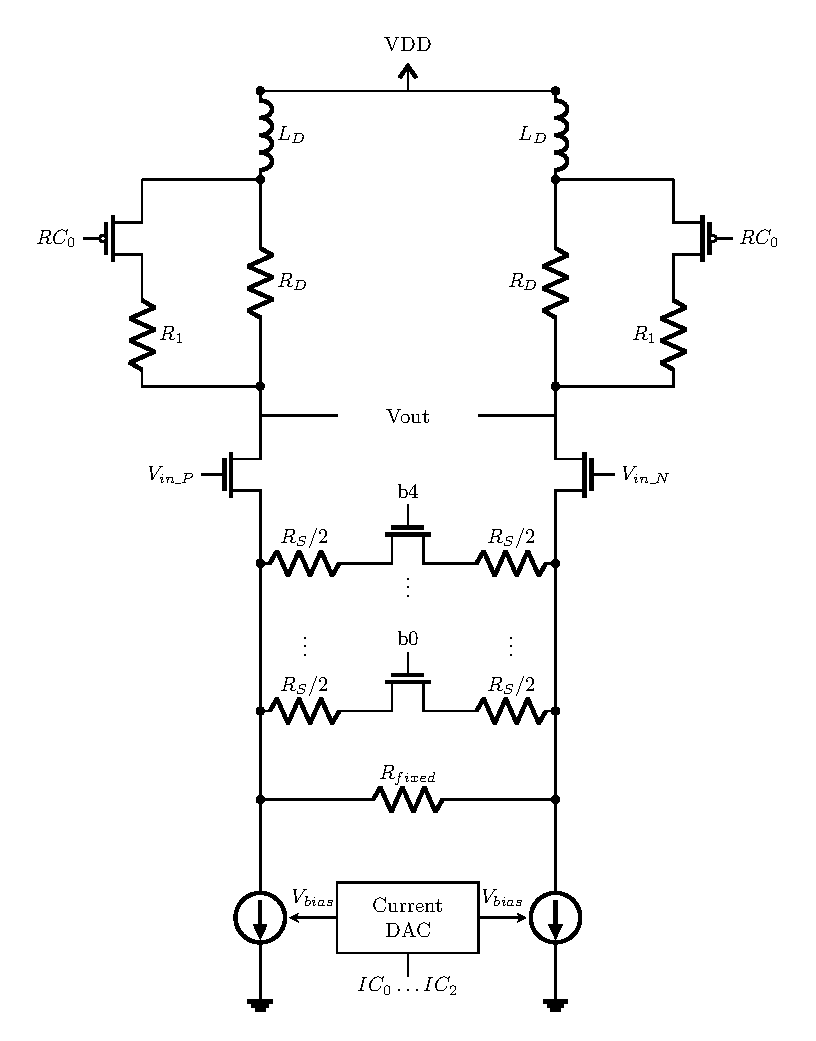
\includegraphics[width=0.45\textwidth]{img/Termination_VGA_img/vga_sch5.pdf} % Replace with vga_sch.pdf
    \caption{Schematic of the proposed Variable Gain Amplifier.}
    \label{fig:vga_schematic}
\end{figure}

\subsection{Detailed Design Procedure}

\subsubsection*{Gain Control via Source Degeneration}
To meet the system specifications, the Variable Gain Amplifier (VGA) is designed to provide a discrete, programmable gain range spanning from 1~dB to 7~dB, with a uniform step size of 1.5~dB. 

The voltage gain of the VGA is discretely tuned by altering the effective source degeneration resistance ($R_S$). The degeneration network consists of a fixed base resistor ($R_{fixed}$) in parallel with a 4-bit coarse array ($b_0$ to $b_3$) for gain stepping, alongside an additional 2-bit fine tuning array ($b_4$ and $b_5$) optimized for corners calibration. The low-frequency differential gain for the half circuit can be approximated as:
\begin{equation}
    A_v \approx \frac{g_m R_D}{1 + g_m (R_S / 2)}
\end{equation}
By progressively activating the parallel coarse branches, the effective value of $R_S$ decreases, which increases the overall transconductance and boosts the voltage gain.

\subsubsection*{Bandwidth Extension via Shunt Peaking}
Driving the large input capacitance ($C_L$) of the DFE introduces a dominant low-frequency pole at the VGA output node ($\omega_p \approx 1 / R_D C_L$). To preserve the 16~GHz bandwidth, a differential shunt peaking inductor ($L_D$) is placed in series with the load resistor ($R_D$). 

The inductor introduces a high-frequency zero into the transfer function ($\omega_z = R_D / L_D$) that delays the capacitive roll-off. The network was designed with an inductive ratio of $m = R_D^2 C_L / L_D = 3.1$ to provide a bandwidth extension ratio (BWER) of $1.57\times$, hence extending the operating frequency range without requiring additional power dissipation.

\subsubsection*{PVT Calibration}
In the Slow-Slow (SS) corner, passive resistance values increases by nearly 20\%. This deviation not only shifts the dominant pole to a lower frequency (degrading operating bandwidth) but also causes an excessive voltage drop across $R_D$. This shifts the output common-mode voltage ($V_{CM}$) downward and compromises the circuit's voltage headroom. 

To mitigate these corner deviations, three distinct calibration networks are implemented to stabilize performance metrics:
\begin{itemize}
    \item \textbf{1-Bit Load Calibration:} A switchable parallel load branch ($R_1$) can be activated in the SS corner. This effectively reduces the total load resistance ($R_{D,eff} = R_D \parallel R_1$), re-centering the bandwidth and restoring the nominal load impedance profile.
    \item \textbf{2-Bit Source Fine Calibration:} Two dedicated fine-tuning resistor branches controlled by the upper control bits ($b_4$ and $b_5$) are included within the source degeneration bank. These branches provide narrow-range adjustments to counteract process variations in the transconductance path without altering the primary coarse gain state definitions.
    \item \textbf{3-Bit Current DAC ($I_{DAC}$):} A binary-weighted current mirror establishes the tail bias current. The DAC consists of a fixed base branch ($I_{base}$) and a 3-bit tuning array (1x, 2x, 4x). Because $V_{CM} = V_{DD} - I_{tail} R_D$, the bias current can be digitally trimmed across corners to preserve a stable $V_{CM}$ and stabilize the input pair $g_m$ regardless of passive resistance drift.
\end{itemize}

\begin{figure}[H]
    \centering
    % --- Left side: Larger Current DAC Schematic ---
    \begin{subfigure}[b]{0.55\textwidth}
        \centering
        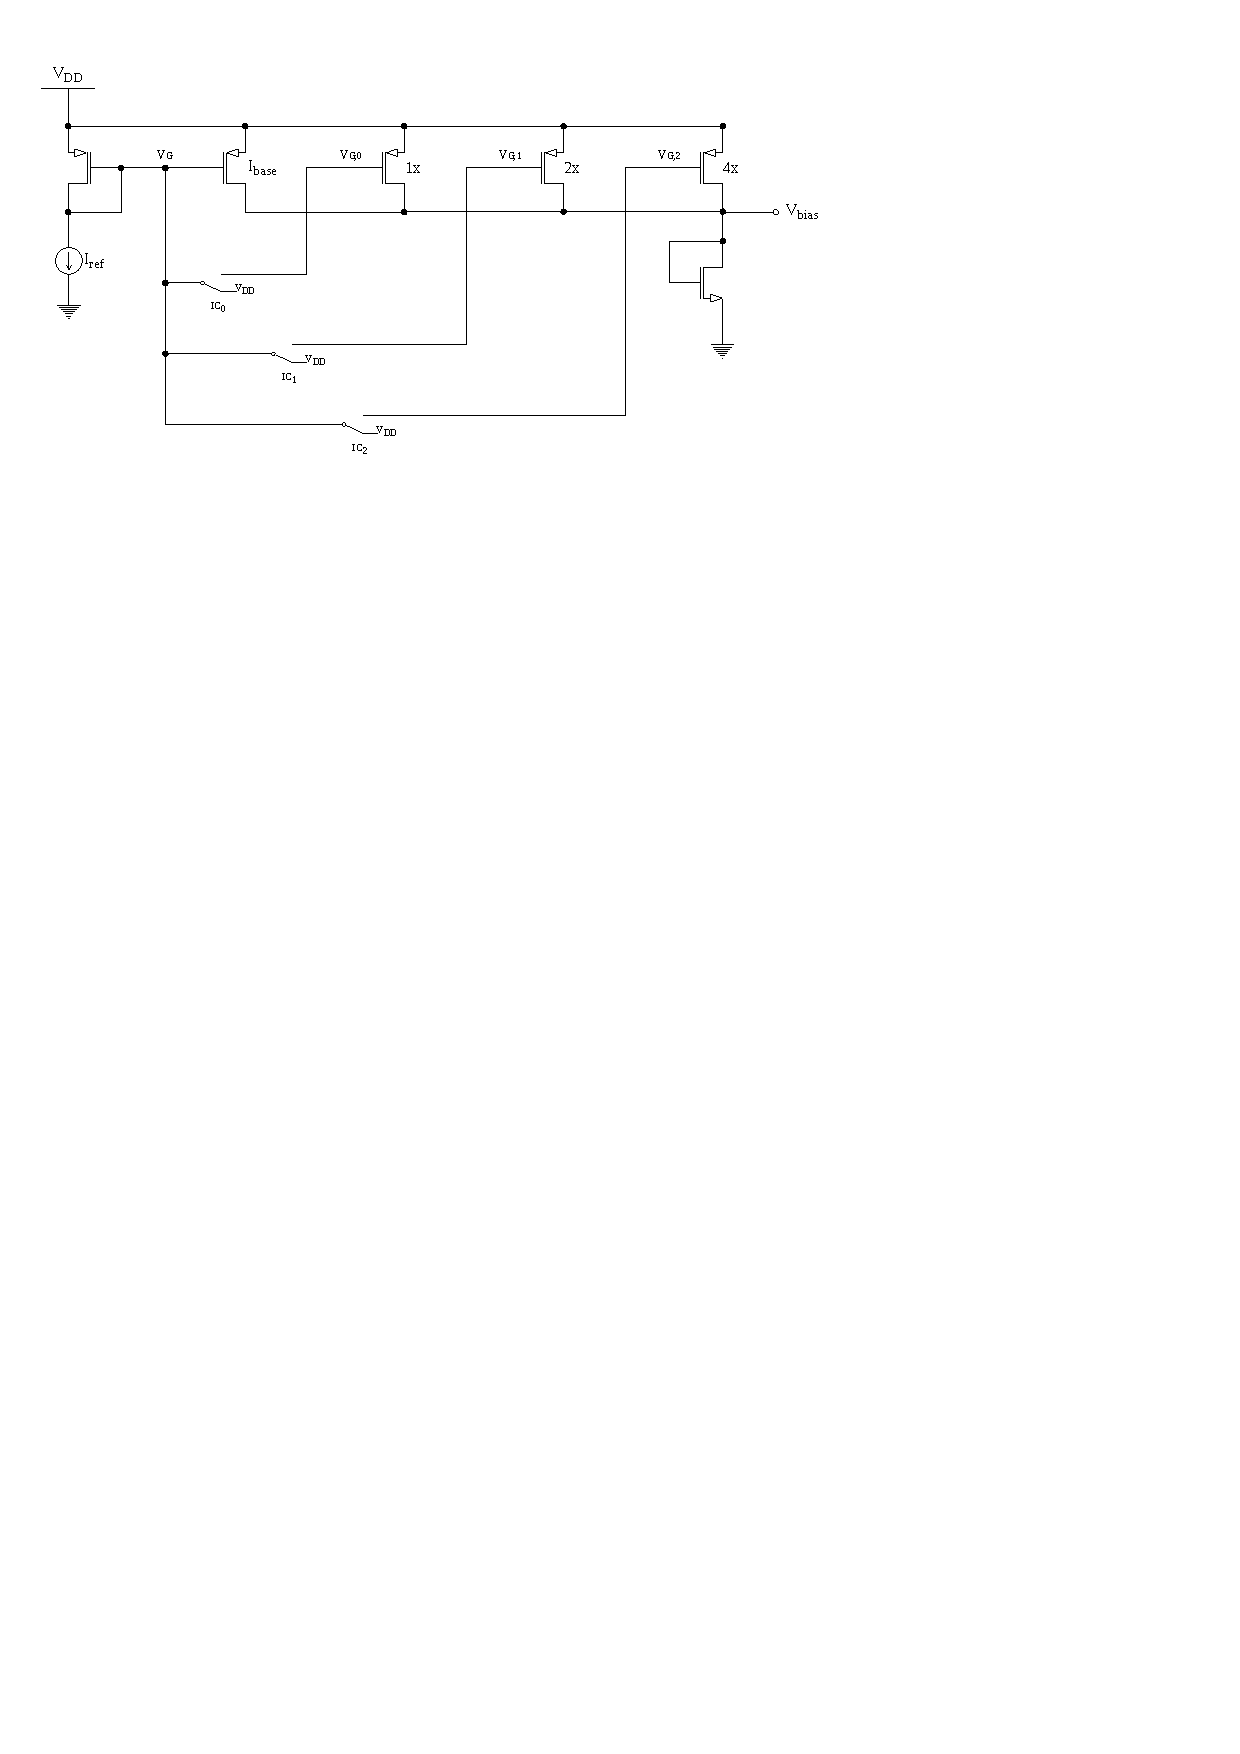
\includegraphics[width=\textwidth]{img/Termination_VGA_img/idac_sch.pdf} % Replace with idac_sch.pdf
        \caption{3-bit binary-weighted Current DAC topology.}
        \label{fig:idac_main}
    \end{subfigure}
    \hfill
    % --- Right side: Smaller 2-Way Switch Schematic ---
    \begin{subfigure}[b]{0.38\textwidth}
        \centering
        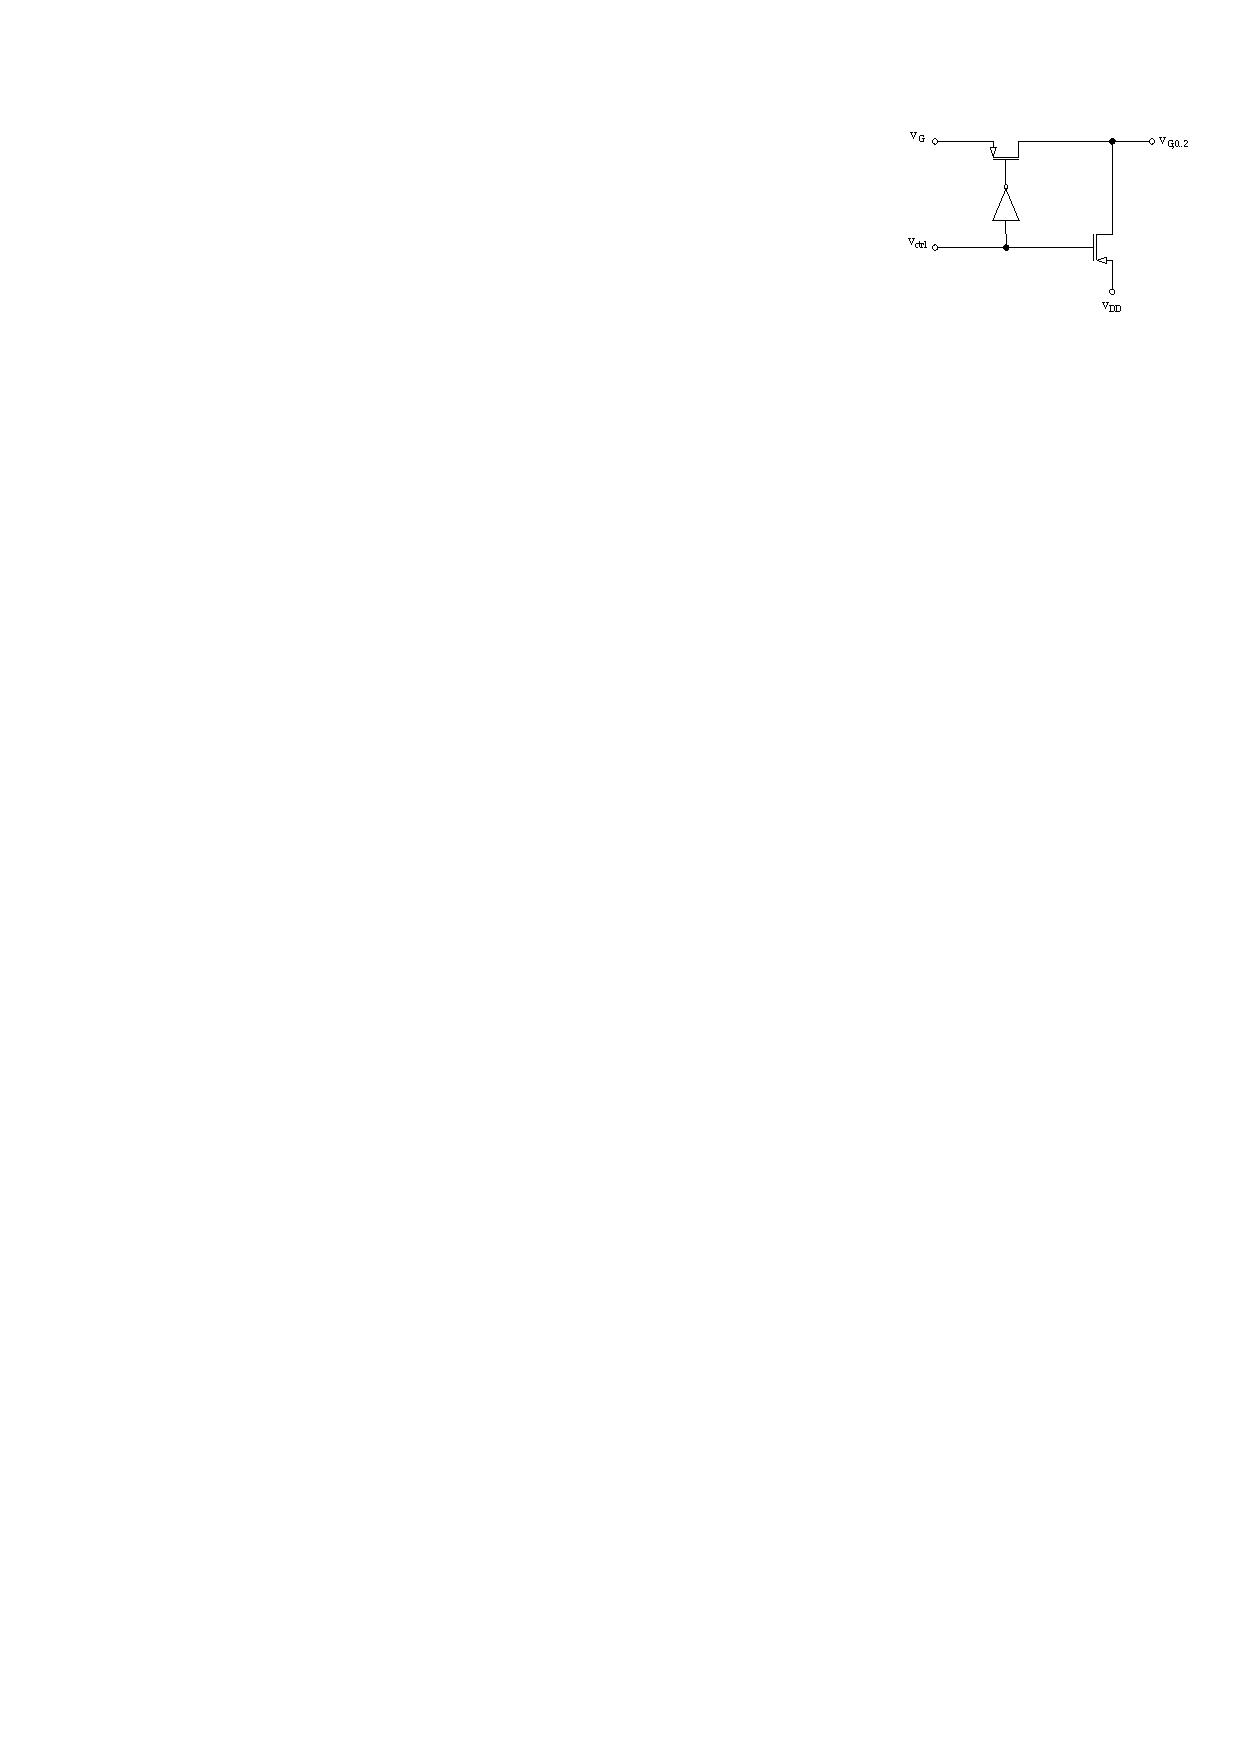
\includegraphics[width=\textwidth]{img/Termination_VGA_img/2wswitch_sch.pdf} % Replace with your 2-way switch image file
        \caption{Transistor-level 2-way switch cell.}
        \label{fig:switch_cell}
    \end{subfigure}
    
    \caption{Schematic configuration of the 3-bit binary-weighted Current DAC.}
    \label{fig:idac_schematic_full}
\end{figure}

\subsection{Implementation and Simulation Results}

\subsubsection*{Differential Peaking Coil Design}
To implement the shunt peaking inductors ($L_D$) compactly, a symmetric differential octagonal coil was designed utilizing the top metal layers to maximize the quality factor. The coil was simulated and extracted using the EMX 3D electromagnetic solver. The physical dimensions and the extracted post-layout parameters are summarized in Table \ref{tab:vga_coil_dims}. 

% --- ROW 1: Layout Image and Dimensions Table Side-by-Side ---
\begin{figure}[H]
    \centering
    % Left side: Layout Image
    \begin{minipage}[c]{0.45\textwidth}
        \centering
        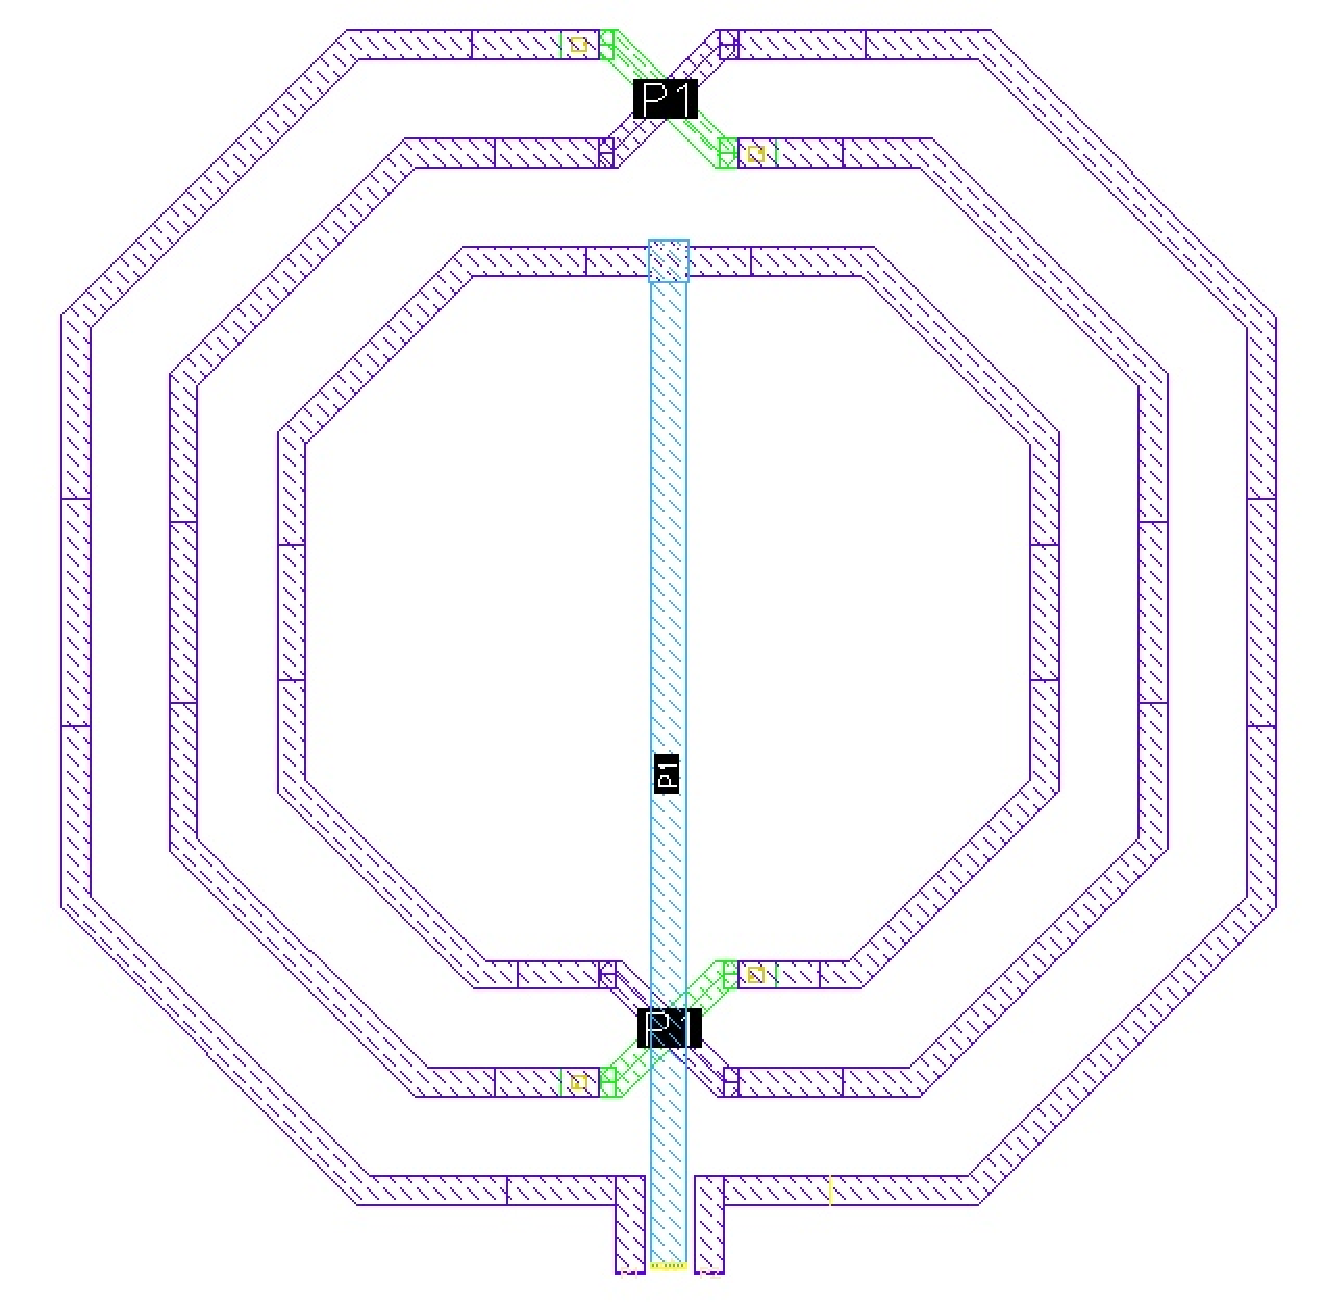
\includegraphics[width=\textwidth]{img/Termination_VGA_img/diff_ind.pdf} % Replace with VGA Coil Layout
        \caption{Differential VGA coil layout.}
        \label{fig:vga_coil_layout}
    \end{minipage}\hfill
    % Right side: Dimensions Table
    \begin{minipage}[c]{0.45\textwidth}
        \centering
        \captionof{table}{VGA Peaking Coil Dimensions}
        \label{tab:vga_coil_dims}
        \begin{tabular}{@{}ll@{}}
            \toprule
            \textbf{Parameter} & \textbf{Value} \\ 
            \midrule
            Outer Diameter ($OD$) & 106.8 $\mu$m \\
            Inner Diameter ($ID$) & 63.8 $\mu$m \\
            Trace Width ($W$)     & 2.5 $\mu$m \\ 
            Turn Spacing ($S$)    & 7 $\mu$m \\
            Number of Turns ($N$) & 3 \\ 
            \bottomrule
        \end{tabular}
    \end{minipage}
\end{figure}

\vspace{0.4cm} % Optional: adds a little breathing room between sections

% --- ROW 2: 1x2 Figure for Inductance and Quality Factor Plots ---
\begin{figure}[H]
    \centering
    \begin{subfigure}[b]{0.48\textwidth}
        \centering
        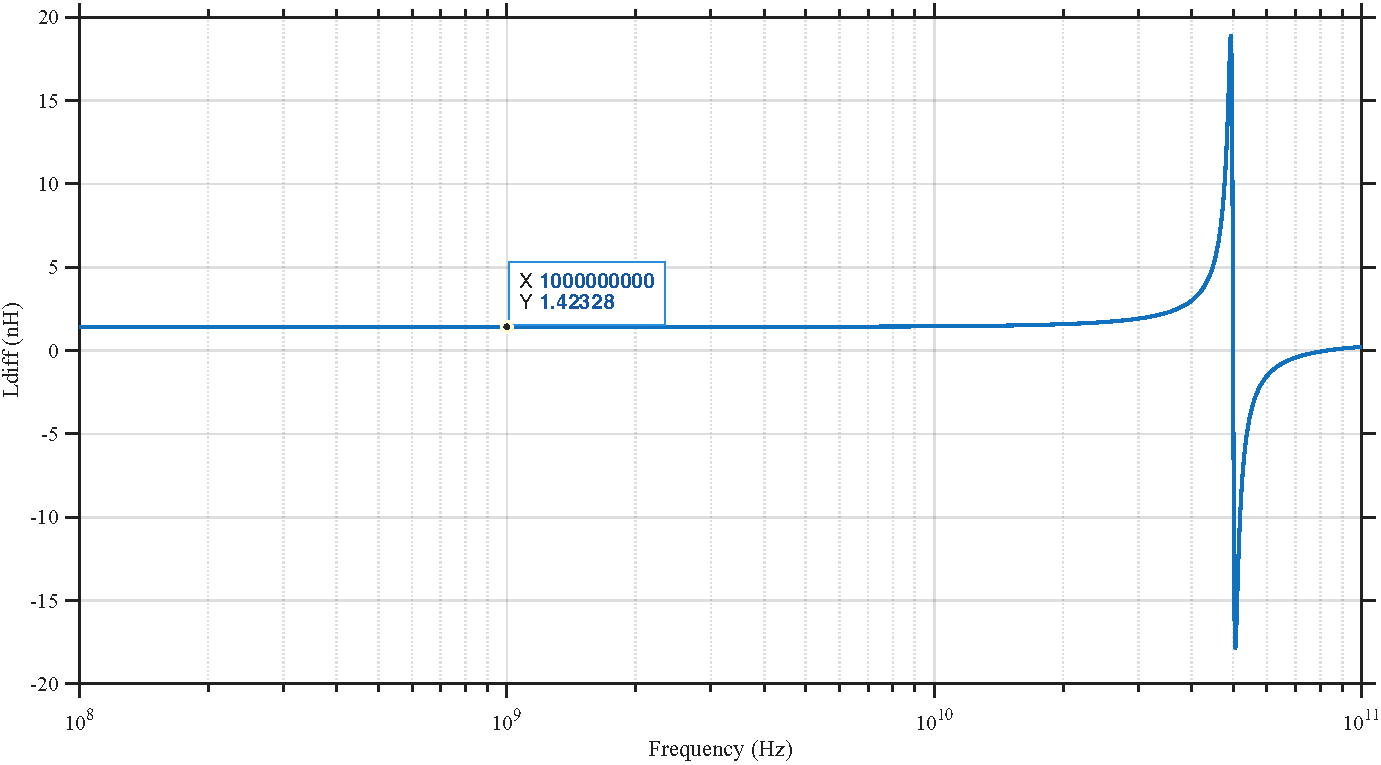
\includegraphics[width=\textwidth]{img/Termination_VGA_img/Ldiff.pdf} % Replace with L plot
        \caption{Extracted Inductance ($L_D$)}
        \label{fig:vga_coil_L}
    \end{subfigure}
    \hfill
    \begin{subfigure}[b]{0.48\textwidth}
        \centering
        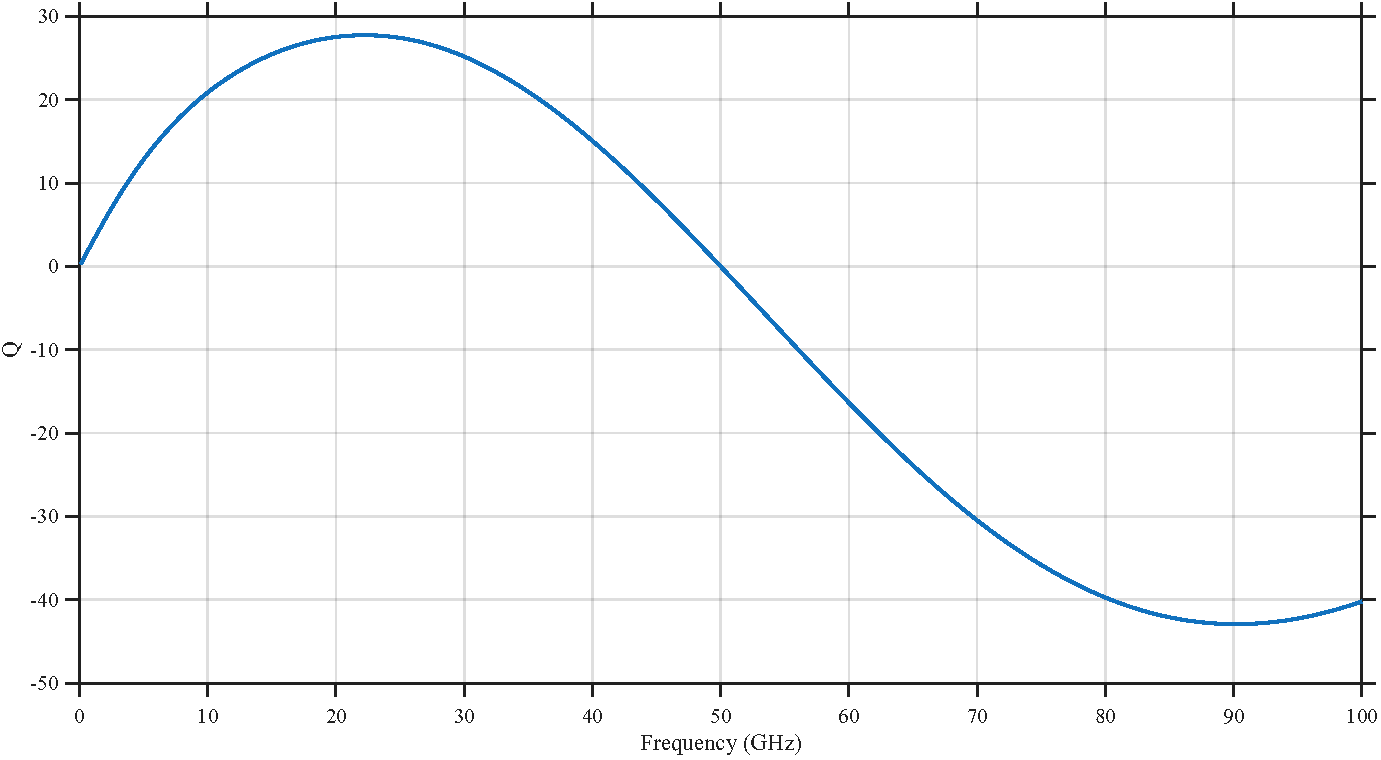
\includegraphics[width=\textwidth]{img/Termination_VGA_img/Qdiff.pdf} % Replace with Q plot
        \caption{Quality Factor ($Q$)}
        \label{fig:vga_coil_Q}
    \end{subfigure}
    \caption{EMX extraction results for the VGA shunt peaking coil across frequency.}
    \label{fig:vga_coil_emx}
\end{figure}

% --- ROW 3: Small Table for Extracted Results ---
\begin{table}[H]
    \centering
    \caption{VGA Peaking Coil: Extracted Performance Metrics}
    \label{tab:vga_coil_results}
    \begin{tabular}{@{}ll@{}}
        \toprule
        \textbf{Parameter} & \textbf{Value} \\ 
        \midrule
        Extracted Inductance ($L_D$ @ 16 GHz) & 1.4 nH \\ 
        Quality Factor ($Q$ @ 16 GHz)         & 26 \\ 
        Self-Resonant Frequency (SRF)         & 50 GHz \\ 
        \bottomrule
    \end{tabular}
\end{table}

\subsubsection*{Gain Steps and AC Performance}
The simulation framework and configuration for the test bench setup are illustrated in Figure~\ref{fig:vga_testbench}. 
The VGA was simulated across its entire discrete tuning range. Figure~\ref{fig:gain_steps} demonstrates the AC response of the five programmed 
gain configurations. The shunt peaking reliably maintains a flat magnitude response well beyond the 16~GHz requirement across all gain settings. 
Table~\ref{tab:gain_codes} maps the control states to their corresponding mid-band gain.

\begin{figure}[H]
    \centering
    \framebox{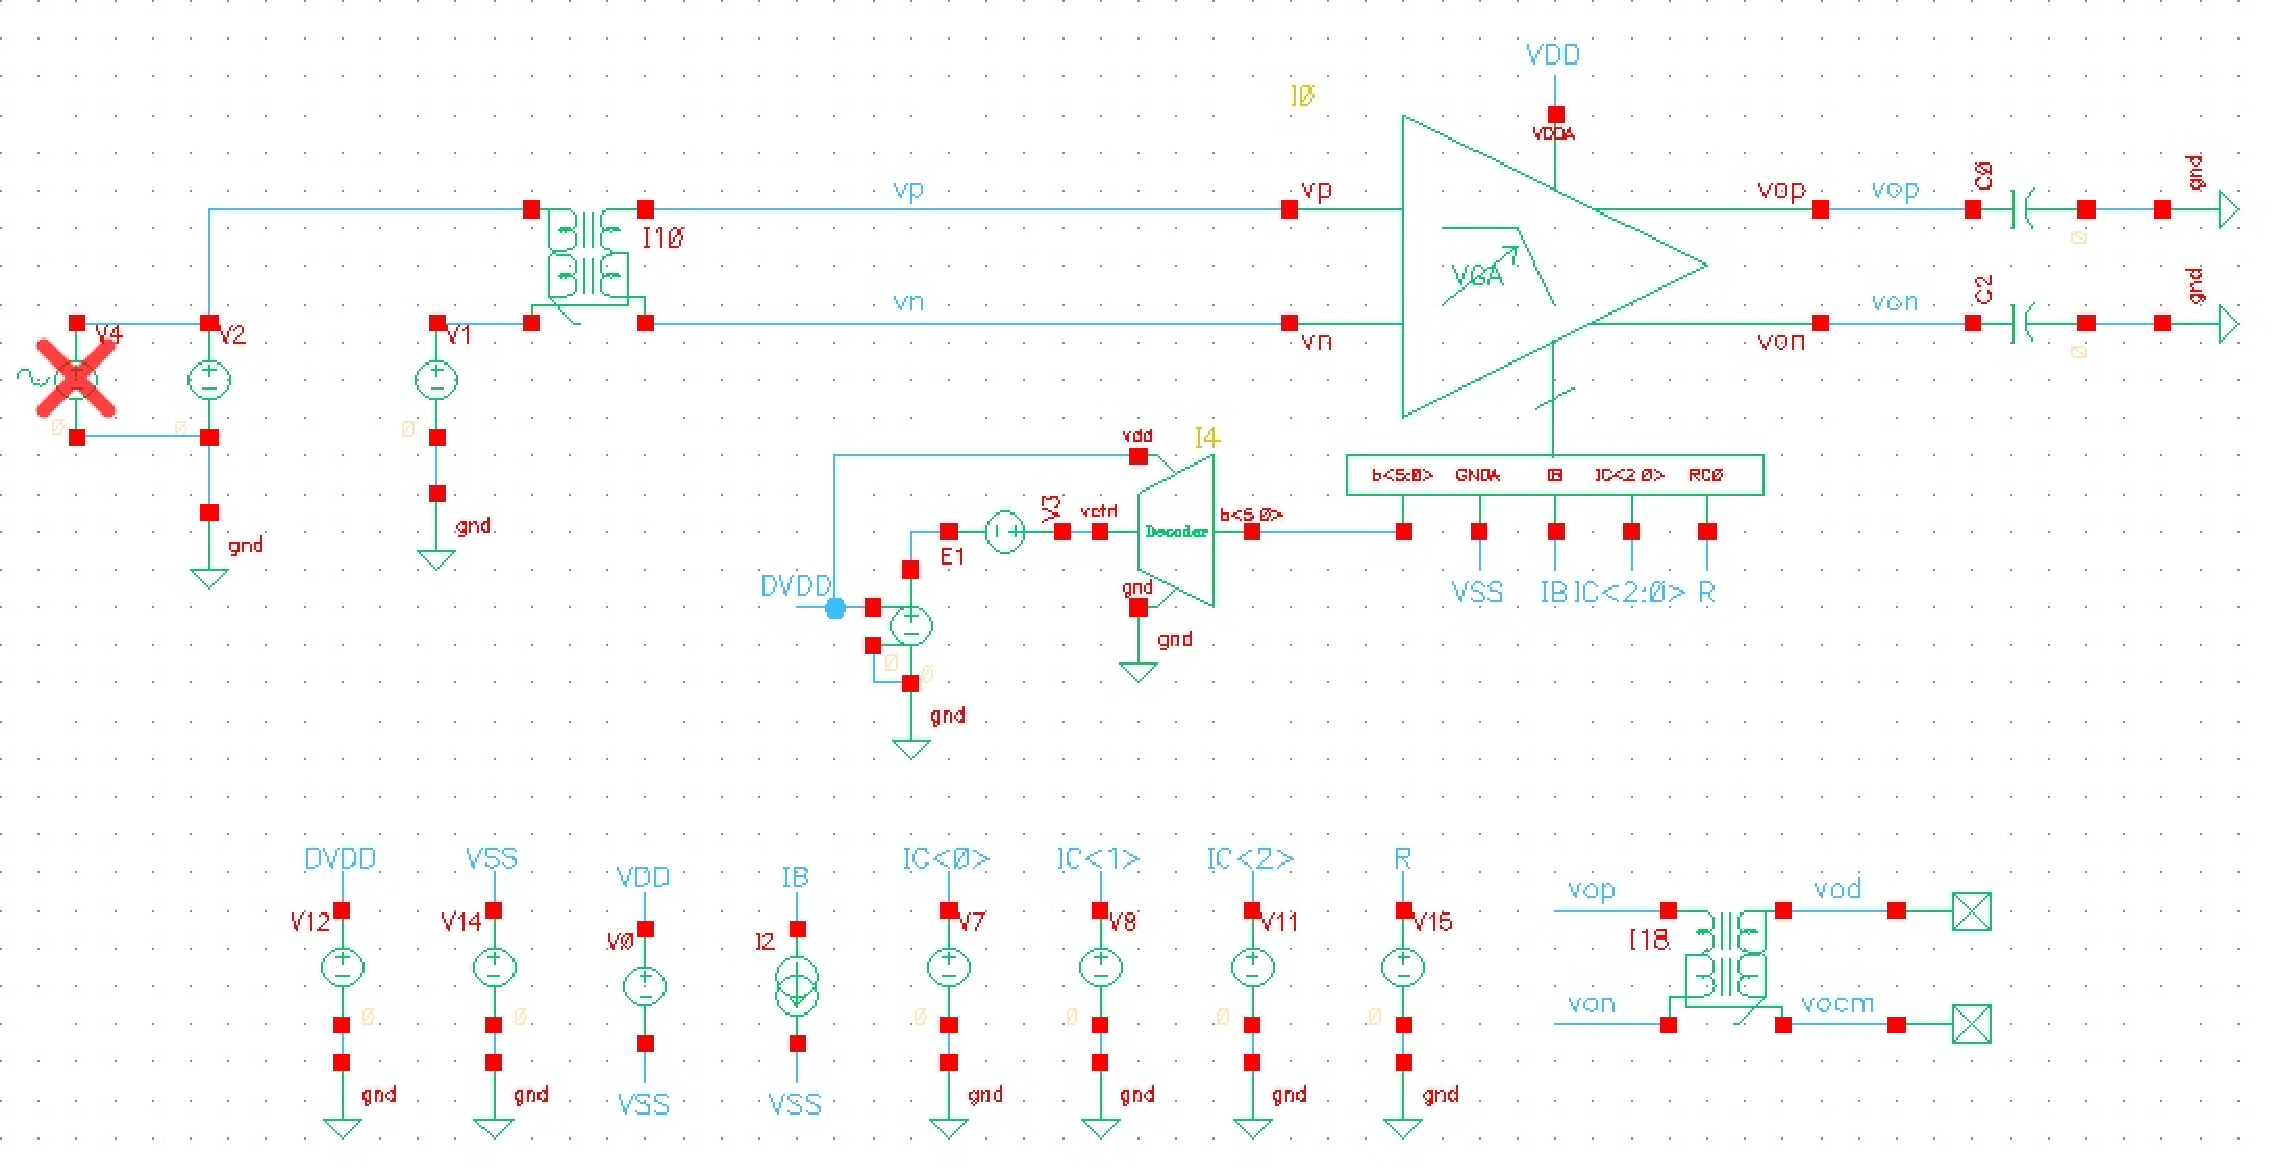
\includegraphics[width=0.95\textwidth]{img/Termination_VGA_img/testbenchvga.pdf}}
    \caption{Simulation test bench schematic configuration for the VGA.}
    \label{fig:vga_testbench}
\end{figure}

\begin{figure}[H]
    \centering
    \framebox{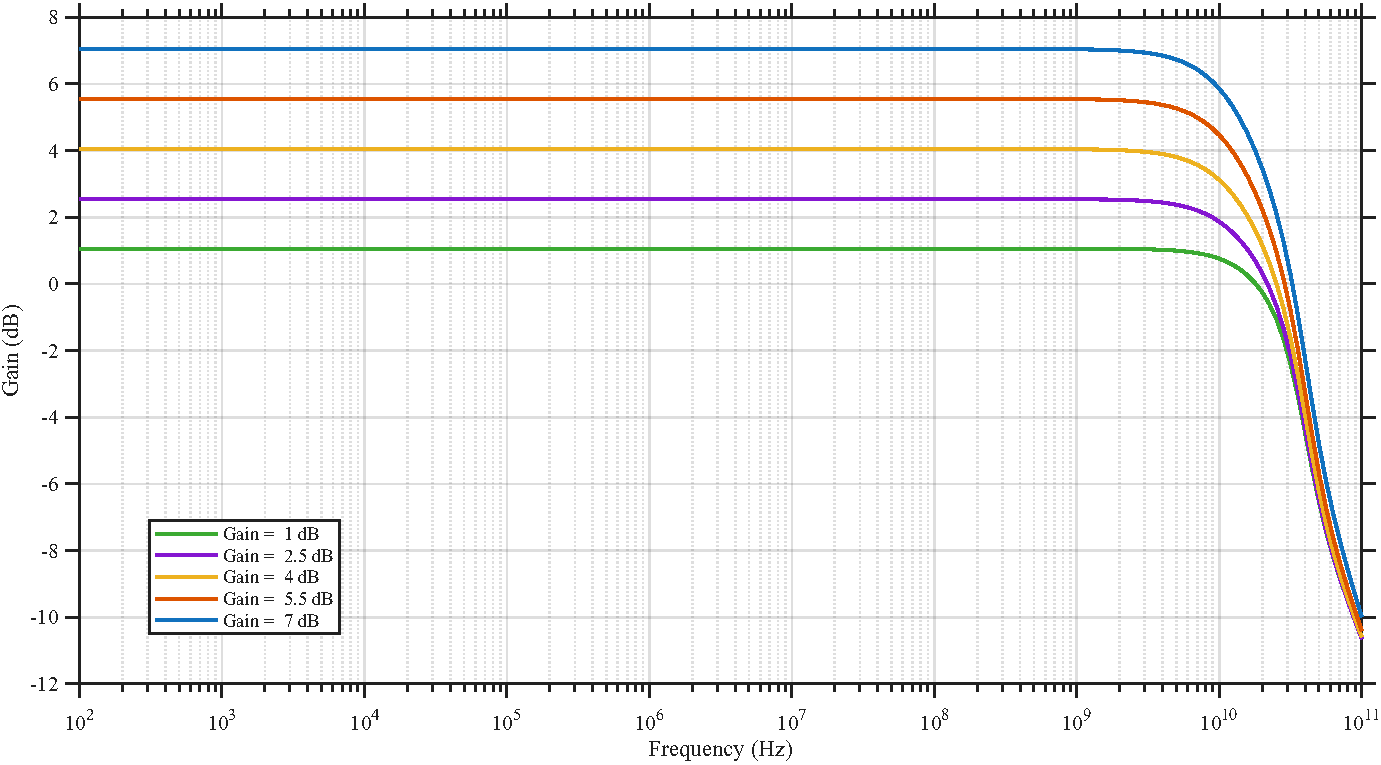
\includegraphics[width=0.9\textwidth]{img/Termination_VGA_img/gain_steps.pdf}} % Replace with gain_steps.pdf
    \caption{VGA AC frequency response illustrating the 5 discrete gain steps.}
    \label{fig:gain_steps}
\end{figure}

\begin{table}[H]
    \centering
    \caption{VGA Gain Steps and Control Configuration}
    \label{tab:gain_codes}
    \begin{tabular}{@{}cc@{}}
        \toprule
        \textbf{Control Code ($b_3 \dots b_0$)} & \textbf{Gain (dB)} \\ 
        \midrule
        0000 & 1.05 \\ 
        0001 & 2.54 \\ 
        0011 & 4.05 \\ 
        0111 & 5.55 \\ 
        1111 & 7.05 \\ 
        \bottomrule
    \end{tabular}
\end{table}

\begin{table}[H]
\centering
\caption{VGA Nominal Performance Parameters}
\label{tab:vga_key_params}
\begin{tabular}{@{}ll@{}}
\toprule
\textbf{Parameter} & \textbf{Nominal Value} \\
\midrule
3-dB Bandwidth ($BW$) & $> 16\,\text{GHz}$ \\
Output Common-Mode Voltage ($V_{CM}$) & $540\,\text{mV}$ \\
Total Current Consumption ($I_{DD}$) & $4.8\,\text{mA}$ \\
\bottomrule
\end{tabular}
\end{table}

\subsubsection*{Linearity Analysis}
To ensure the PAM4 signal integrity is not compromised by amplifier compression, the large-signal linearity of the VGA was evaluated at both the minimum (1~dB) and maximum (7~dB) gain steps. As illustrated in Figure~\ref{fig:vga_linearity}, the linearity profile is heavily dependent on the programmed gain state due to the variable source degeneration architecture.

At the minimum gain setting (1~dB), the maximum source degeneration resistance is applied. This linearizes the effective transconductance of the differential pair, yielding a highly linear transfer characteristic across a broad differential input range ($V_{id} \approx \pm 0.4\,\text{V}$). Consequently, the distortion remains negligible, with the THD staying well below 1\% for typical input amplitudes.

Conversely, at the maximum gain setting (7~dB), the coarse degeneration branches are activated, minimizing the effective source resistance to maximize voltage gain. While this fulfills the dynamic range requirements, the amplifier's response becomes increasingly dominated by the intrinsic nonlinearities of the input transistors. The onset of soft saturation (headroom compression) becomes visible in the voltage transfer curve beyond an input swing of $\pm 0.2\,\text{V}$.

\begin{figure}[H]
    \centering
    \begin{subfigure}[b]{0.48\textwidth}
        \centering
        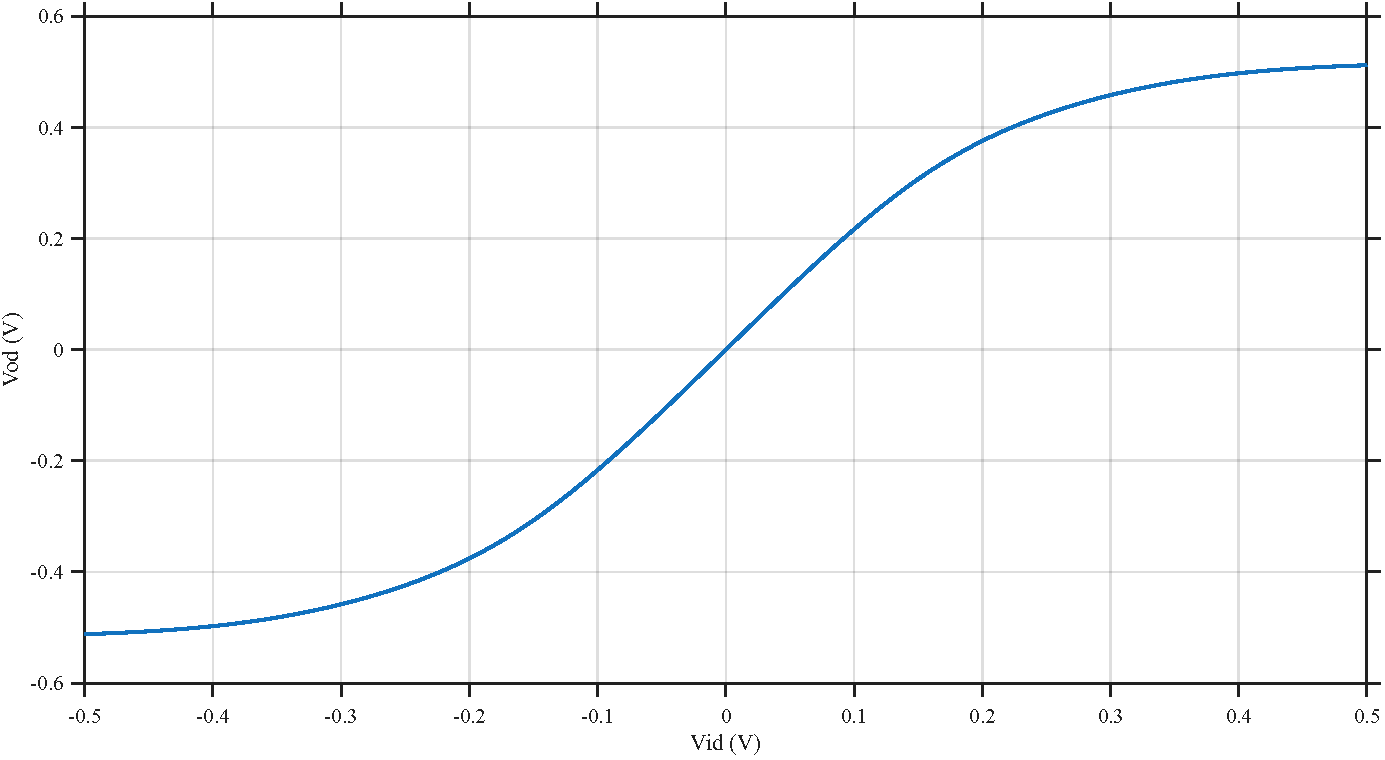
\includegraphics[width=\textwidth]{img/Termination_VGA_img/7db_scurve.pdf} 
        \caption{Voltage Transfer Curve at 7 dB Gain}
        \label{fig:vga_scurve_7db}
    \end{subfigure}
    \hfill
    \begin{subfigure}[b]{0.48\textwidth}
        \centering
        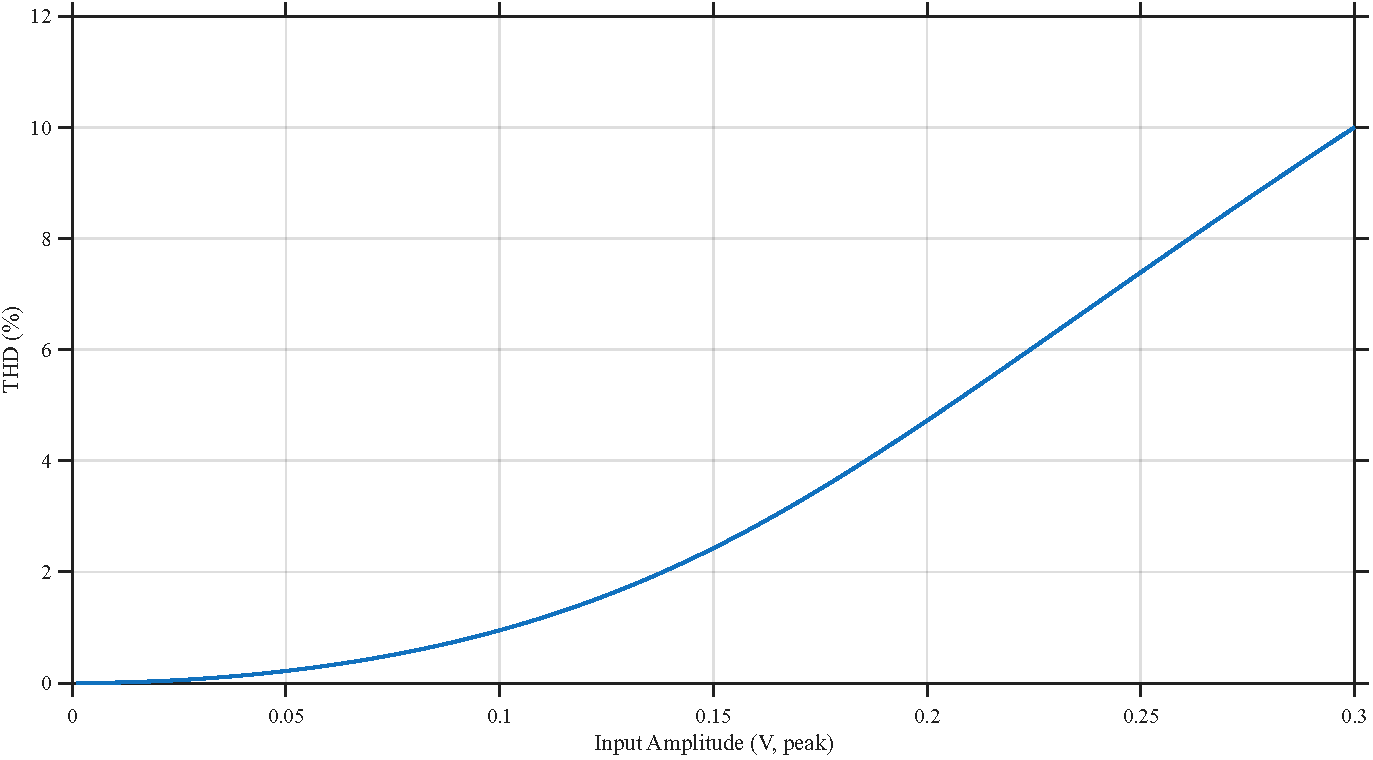
\includegraphics[width=\textwidth]{img/Termination_VGA_img/THD_7db.pdf} 
        \caption{THD Profile at 7 dB Gain}
        \label{fig:vga_thd_7db}
    \end{subfigure}

    \vspace{0.4cm} 

    \begin{subfigure}[b]{0.48\textwidth}
        \centering
        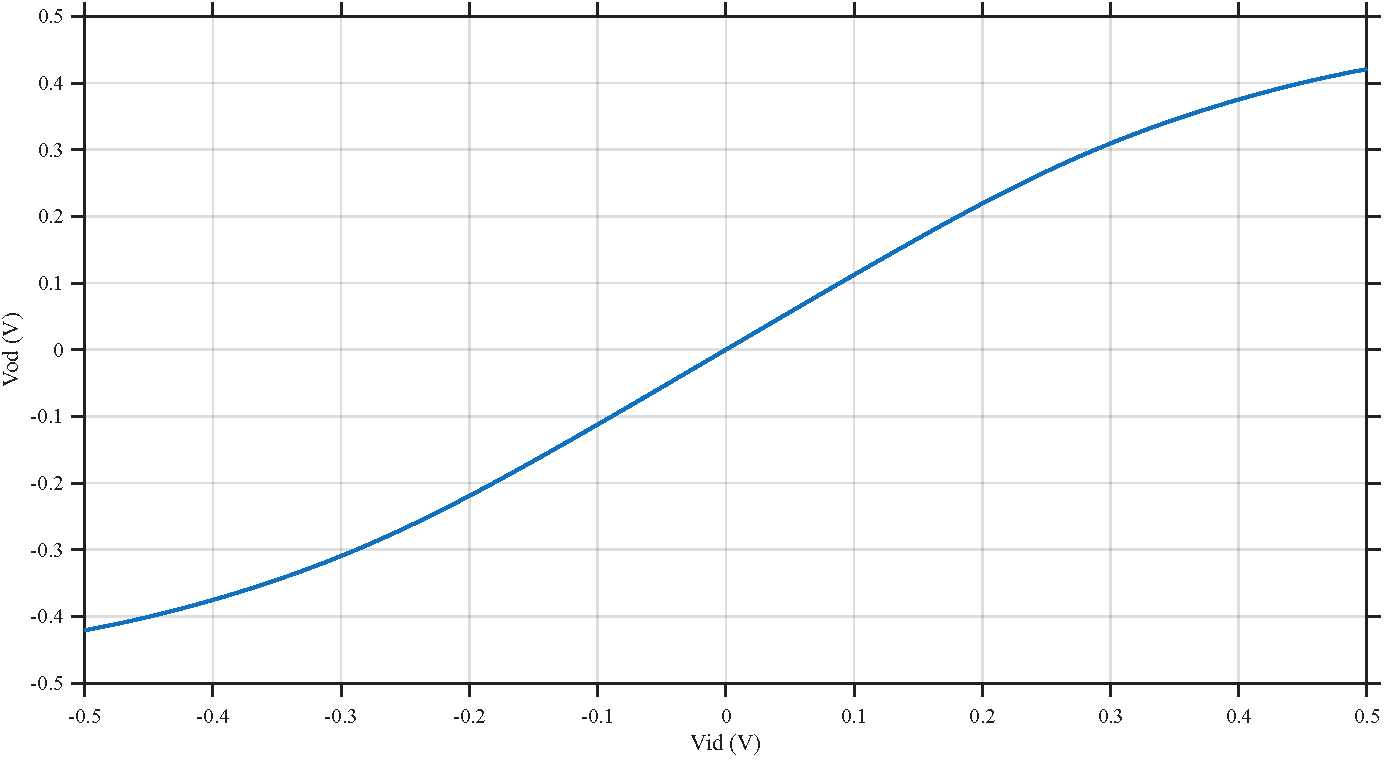
\includegraphics[width=\textwidth]{img/Termination_VGA_img/1db_scurve.pdf} 
        \caption{Voltage Transfer Curve at 1 dB Gain}
        \label{fig:vga_scurve_1db}
    \end{subfigure}
    \hfill
    \begin{subfigure}[b]{0.48\textwidth}
        \centering
        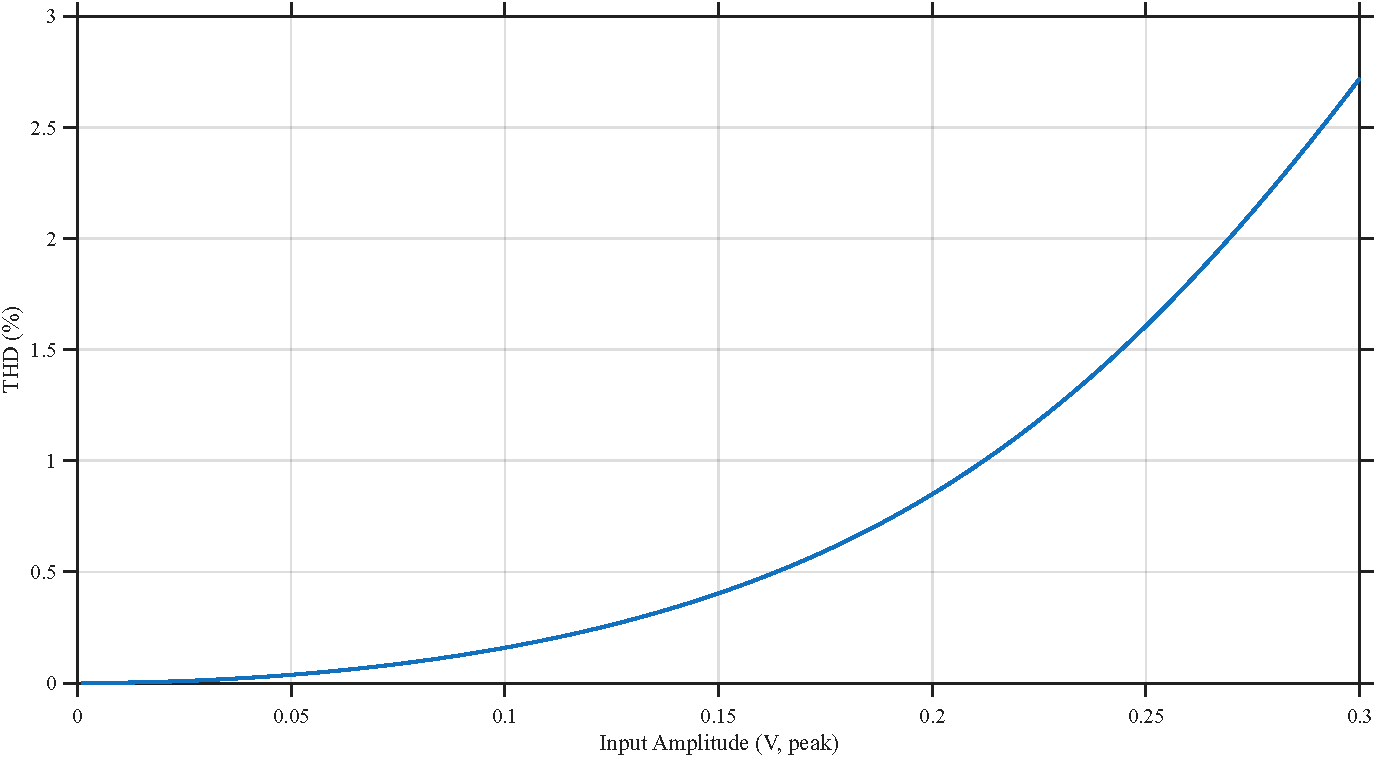
\includegraphics[width=\textwidth]{img/Termination_VGA_img/THD_1db.pdf} 
        \caption{THD Profile at 1 dB Gain}
        \label{fig:vga_thd_1db}
    \end{subfigure}

    \caption{Linearity analysis of the VGA at minimum and maximum gain configurations.}
    \label{fig:vga_linearity}
\end{figure}

This compression behavior directly correlates with the Total Harmonic Distortion (THD) profiles. As summarized in Table~\ref{tab:thd_summary}, 
driving the VGA with a $200\,\text{mV}_{peak}$ signal yields a highly linear response (0.8\% THD) at minimum gain, 
whereas the same input amplitude at maximum gain pushes the THD to approximately 4.8\% due to the amplification of third-order intermodulation products. 
This verifies that the VGA provides adequate voltage headroom and maintains acceptable PAM4 signal integrity within the nominal operating window.

\begin{table}[H]
    \centering
    \caption{Total Harmonic Distortion (THD) vs. Input Amplitude}
    \label{tab:thd_summary}
    \begin{tabular}{@{}lccc@{}}
        \toprule
        \textbf{Gain State} & \textbf{THD @ $100\text{ mV}_{peak}$} & \textbf{THD @ $200\text{ mV}_{peak}$} & \textbf{THD @ $300\text{ mV}_{peak}$} \\ 
        \midrule
        Minimum Gain (1~dB) & $\approx 0.15\%$ & $\approx 0.8\%$ & $\approx 2.7\%$ \\ 
        Maximum Gain (7~dB) & $\approx 1.0\%$ & $\approx 4.8\%$ & $\approx 10.0\%$ \\ 
        \bottomrule
    \end{tabular}
\end{table}

\subsubsection*{PVT Corner Analysis}
A rigorous corner analysis was performed for every discrete gain step (1 dB, 2.5 dB, 4 dB, 5.5 dB, and 7 dB) to validate the effectiveness of 
the calibration networks. A total of 12 corners were simulated for each state, encompassing process variations (Slow-Slow and Fast-Fast), 
supply voltage fluctuations ($\pm 5\%$ VDD), and extreme temperature variations ($-40^\circ\text{C}$ to $125^\circ\text{C}$). 

By engaging the 1-bit $R_1$ load calibration in the SS corners and trimming the tail current via the 3-bit $I_{DAC}$, the VGA was able to maintain its target gain profile, bandwidth, and common-mode voltage across all severe PVT shifts with minimum variations.

\begin{figure}[H]
    \centering
    \begin{subfigure}[b]{0.48\textwidth}
        \centering
        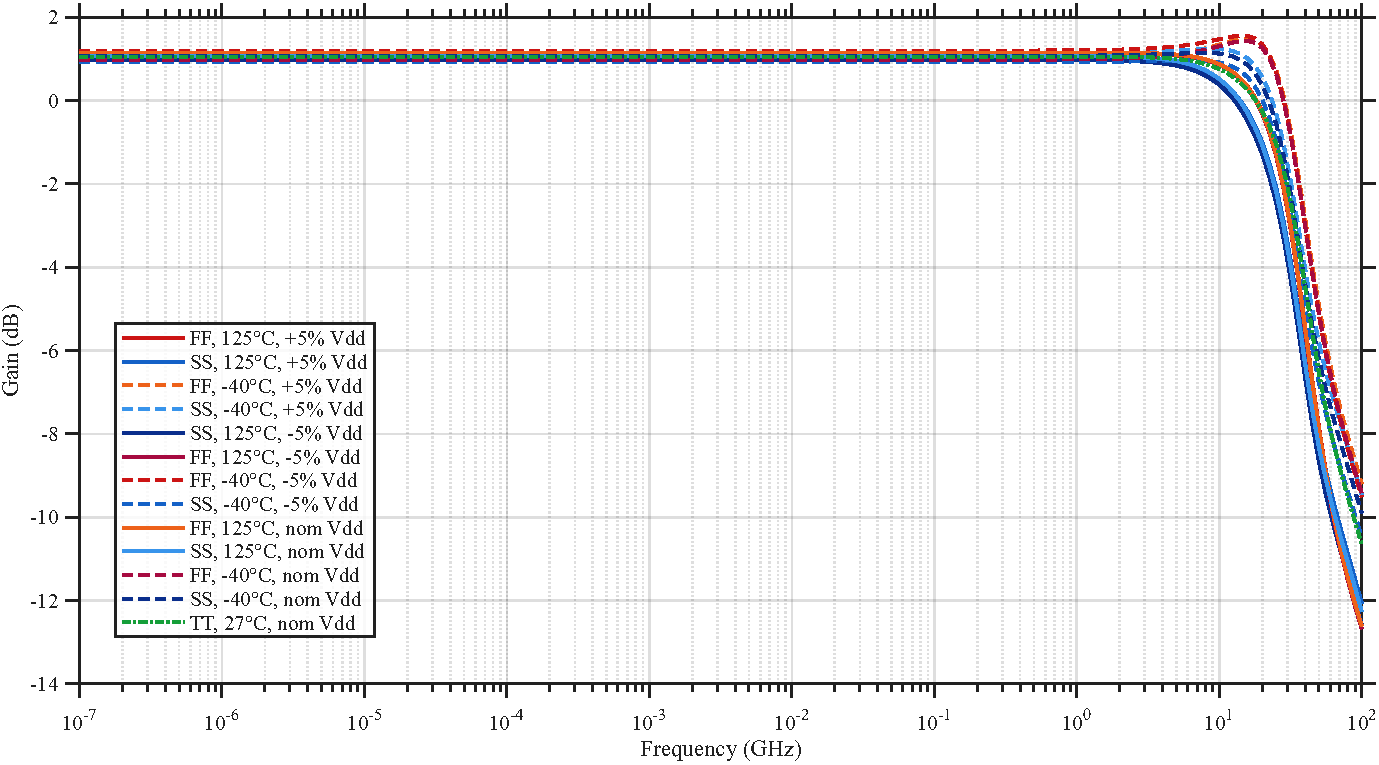
\includegraphics[width=\textwidth]{img/Termination_VGA_img/1db_corners.pdf} % Replace with 1st step e.g., 1db_corners.pdf
        \caption{1 dB Gain Step}
        \label{fig:vga_corner_1db}
    \end{subfigure}
    \hfill
    \begin{subfigure}[b]{0.48\textwidth}
        \centering
        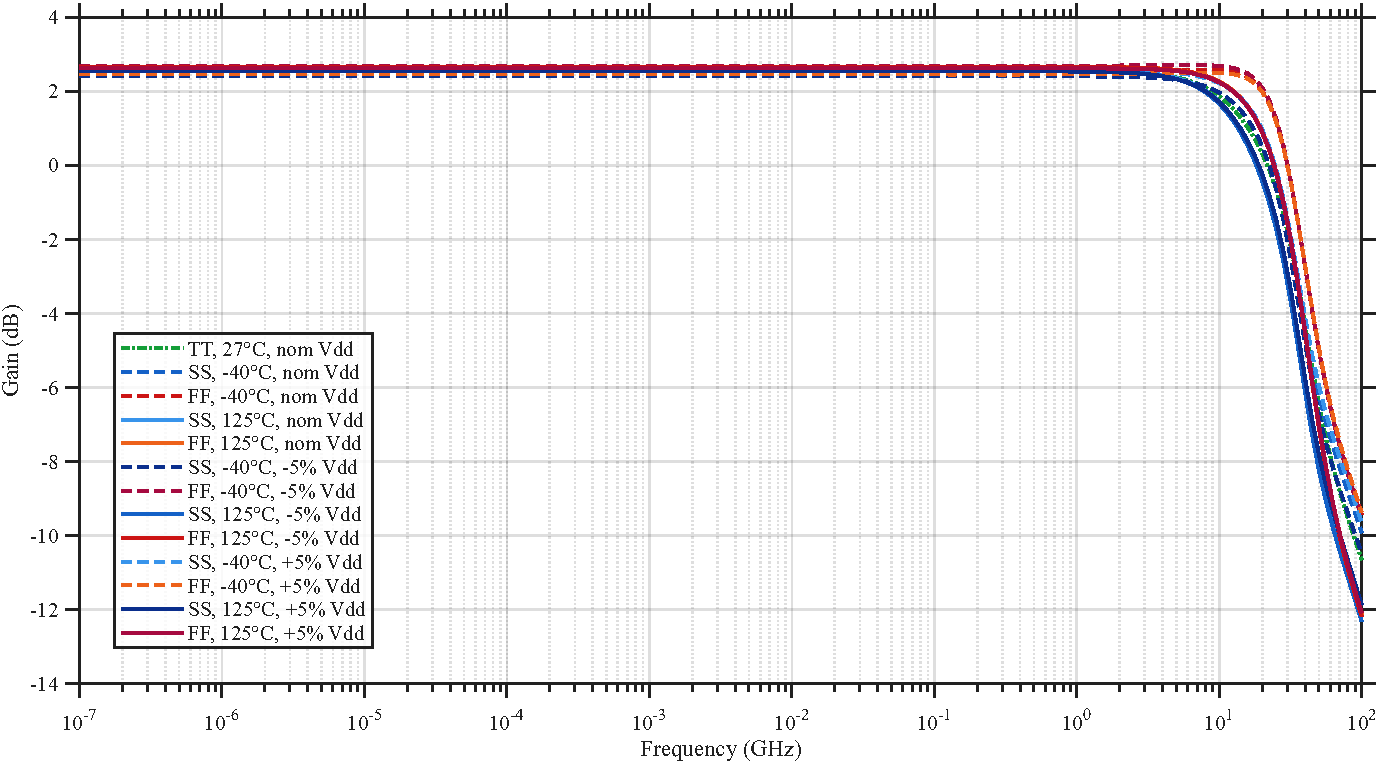
\includegraphics[width=\textwidth]{img/Termination_VGA_img/2_5db_corners.pdf} % Replace with 2nd step
        \caption{2.5 dB Gain Step}
        \label{fig:vga_corner_3db}
    \end{subfigure}

    \vspace{0.4cm} % Space between Row 1 and Row 2

    % --- Row 2 ---
    \begin{subfigure}[b]{0.48\textwidth}
        \centering
        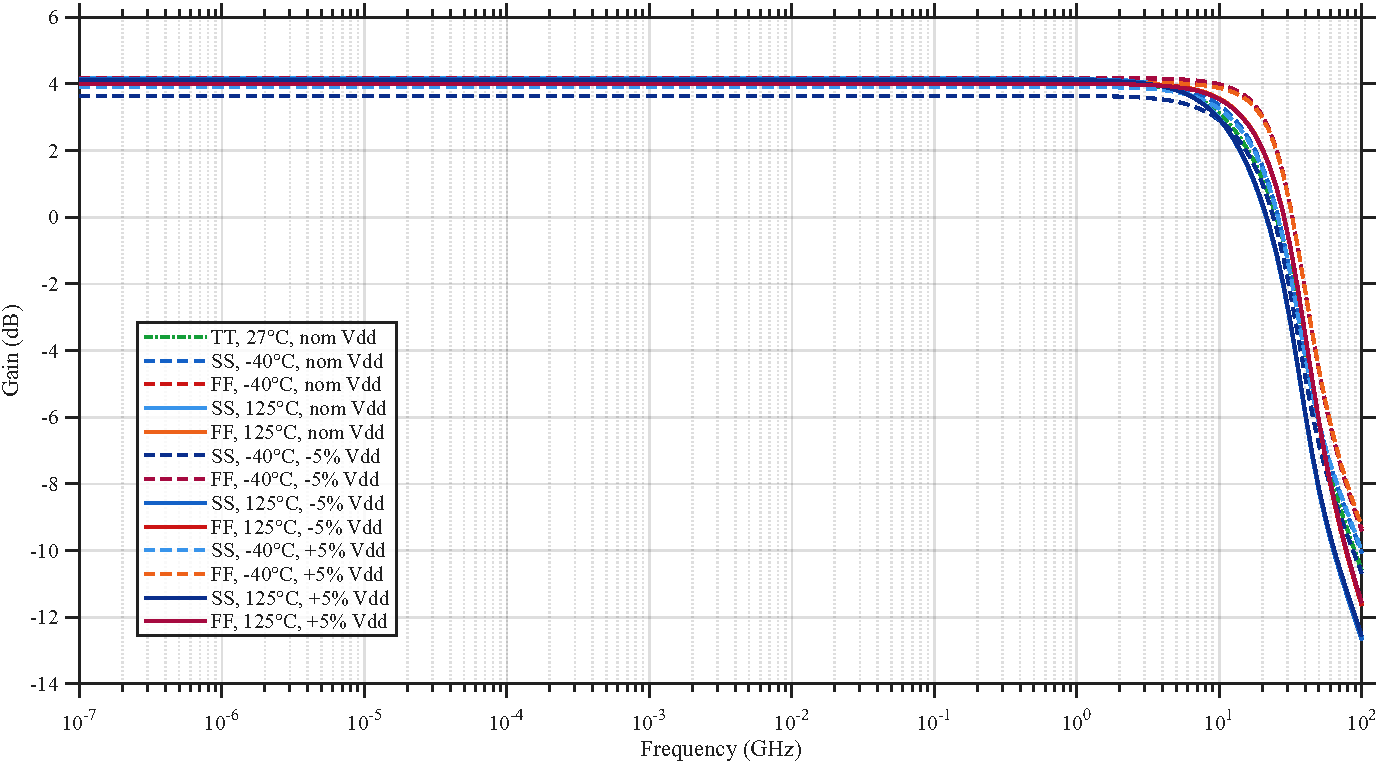
\includegraphics[width=\textwidth]{img/Termination_VGA_img/4db_corners.pdf} % Replace with 3rd step
        \caption{4 dB Gain Step}
        \label{fig:vga_corner_5db}
    \end{subfigure}
    \hfill
    \begin{subfigure}[b]{0.48\textwidth}
        \centering
        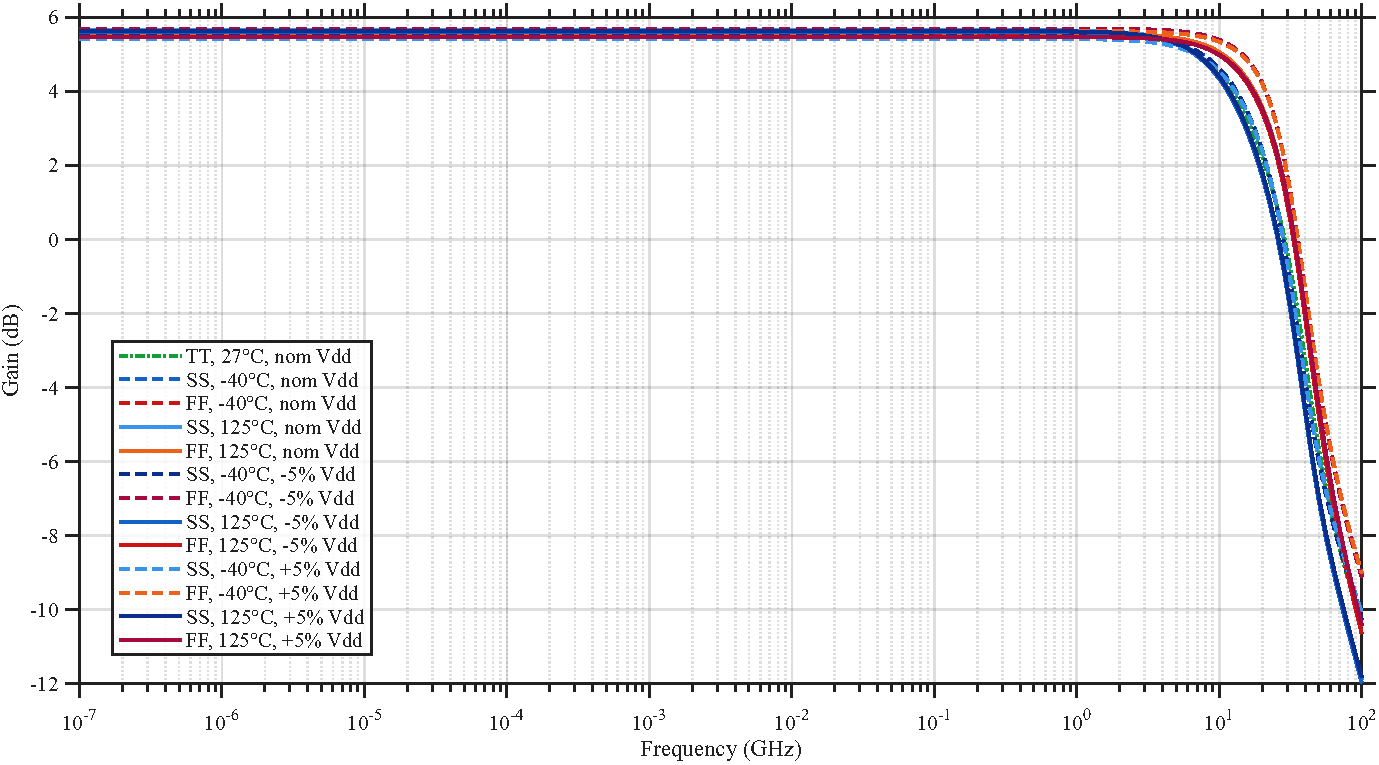
\includegraphics[width=\textwidth]{img/Termination_VGA_img/5_5db_corners.pdf} % Replace with 4th step e.g., 7db_corners.pdf
        \caption{5.5 dB Gain Step}
        \label{fig:vga_corner_7db}
    \end{subfigure}

    \vspace{0.4cm} % Space between Row 2 and Row 3

    % --- Row 3 (Centered single plot) ---
    \begin{subfigure}[b]{0.48\textwidth}
        \centering
        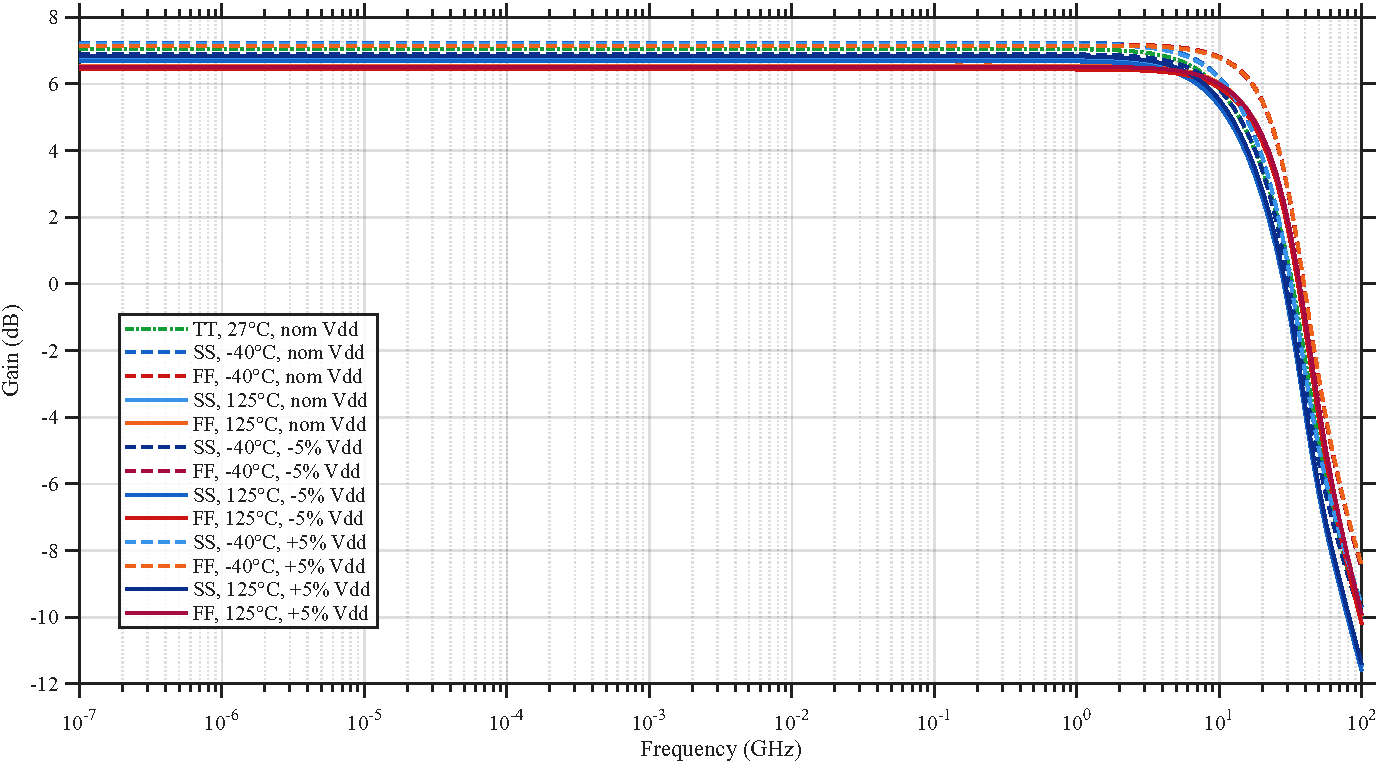
\includegraphics[width=\textwidth]{img/Termination_VGA_img/7db_corners.pdf} % Replace with 5th step
        \caption{7 dB Gain Step}
        \label{fig:vga_corner_9db}
    \end{subfigure}

    \caption{PVT corner simulation results across all gain steps.}
    \label{fig:vga_corners}
\end{figure}

\begin{table}[H]
    \centering
    \caption{Summary of VGA PVT Corner Simulation Performance}
    \label{tab:vga_corner_summary}
    \begin{tabular}{@{}ll@{}}
        \toprule
        \textbf{Performance Metric} & \textbf{Variation} \\
        \midrule
        Common-Mode Voltage ($V_{CM}$) & $\sim \pm 20\,\text{mV}$ \\
        DC Gain  & $< \pm 0.6\,\text{dB}$ \\
        3-dB Bandwidth ($BW$) & $> 16\,\text{GHz}$ \\
        Current Consumption  & $< 5.5\,\text{mA}$ \\
        Device Operating Region & All  transistors remain in saturation \\
        \bottomrule
    \end{tabular}
\end{table}

\subsection{Layout Implementation and Post-Layout Verification}

A symmetric floorplan was enforced across the differential signaling path to preserve circuit balance and minimise parasitics to ensure optimal overall high-frequency performance.

\subsubsection{Floorplan and Physical Layout}
As shown in Figure \ref{fig:vga_layouts}, the components are arranged systematically to preserve structural symmetry. The programmable resistor bank (R-bank) is placed directly adjacent to the active core stage source nodes. This layout strategy keeps the sensitive source degeneration routing as short and symmetric as possible, preventing interconnect parasitics from shifting the intended impedance characteristics.

\begin{figure}[H]
    \centering
    \begin{subfigure}[b]{0.48\textwidth}
        \centering
        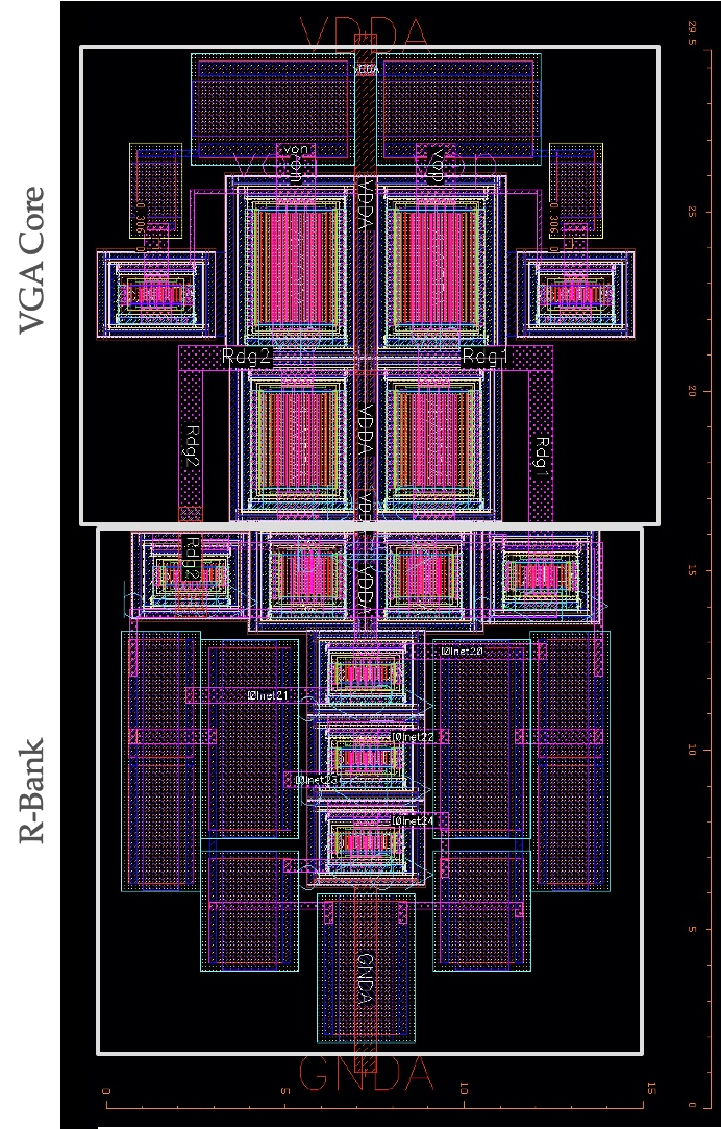
\includegraphics[width=\textwidth]{img/Termination_VGA_img/vgalayoutwoind.pdf}
        \caption{VGA Core Layout (Pre-Coil)}
        \label{fig:vga_core_layout}
    \end{subfigure}
    \hfill
    \begin{subfigure}[b]{0.48\textwidth}
        \centering
        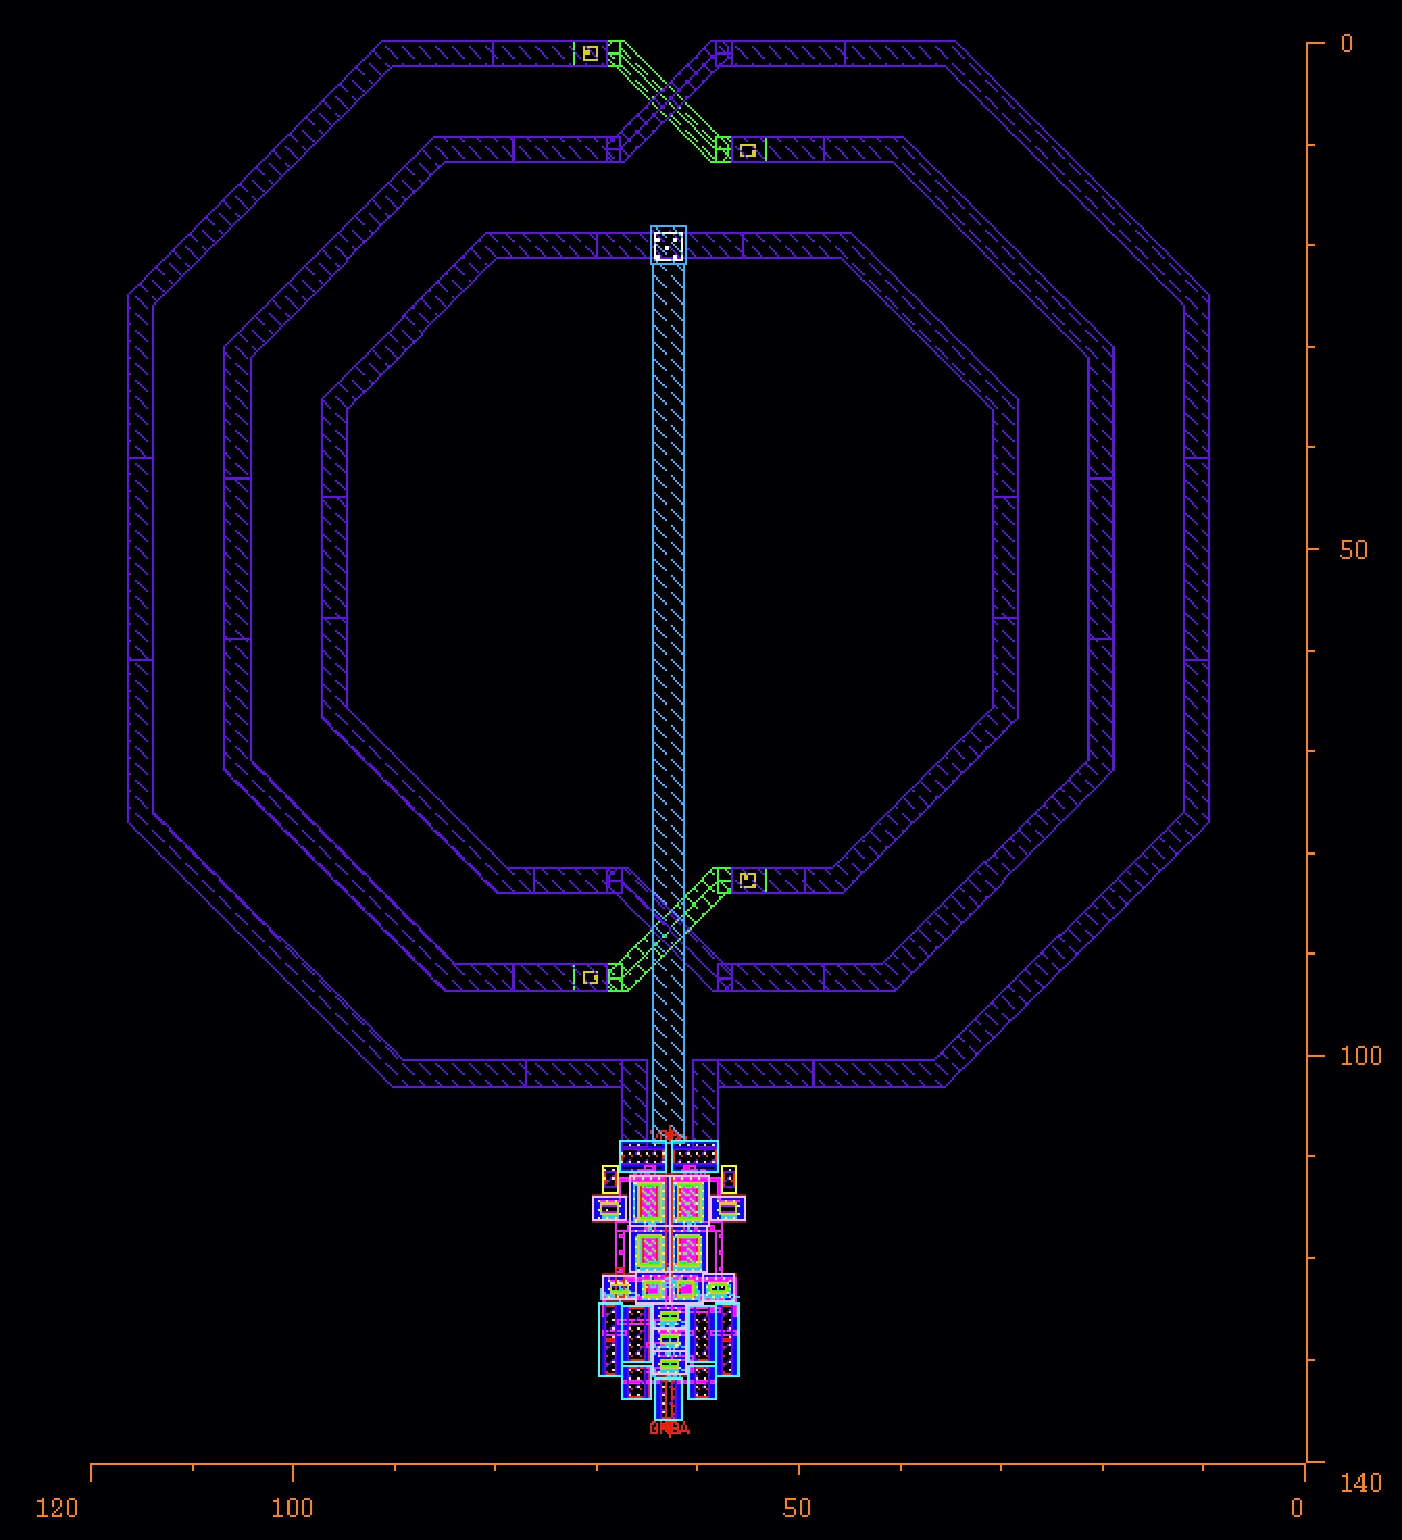
\includegraphics[width=\textwidth]{img/Termination_VGA_img/vga_layout_post_black.pdf}
        \caption{Complete VGA Layout}
        \label{fig:vga_complete_layout}
    \end{subfigure}
    \caption{Physical layout implementation of the VGA before and after inductor integration.}
    \label{fig:vga_layouts}
\end{figure}

\subsubsection*{Post-Layout Extraction (PEX) Simulation}
To validate the robustness of the physical design, Post-Layout Extraction (PEX) was performed to capture the parasitic resistances and capacitances (RC) introduced by the metal routing, via stacks, and device placement. Figure \ref{fig:pex_vs_sch} compares the fully extracted PEX netlist simulation against the ideal pre-layout schematic response. The comparison confirms that the layout successfully preserves the required bandwidth and gain profiles with minimal parasitic degradation.

\begin{figure}[H]
    \centering
    \framebox{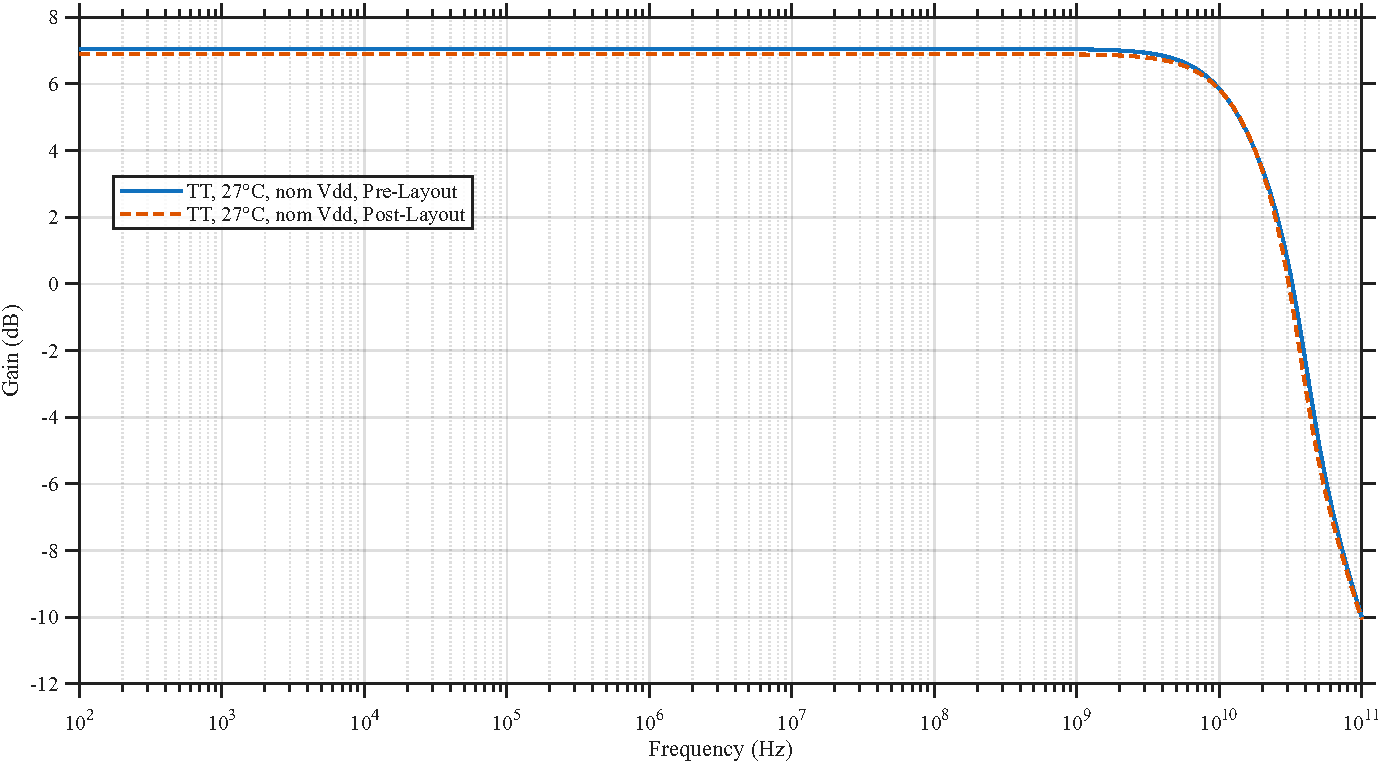
\includegraphics[width=0.9\textwidth]{img/Termination_VGA_img/7db_postLayout.pdf}}
    \caption{Post-layout AC frequency response verification at the maximum gain step.}
    \label{fig:pex_vs_sch}
\end{figure}

\subsection{Front-End Chain Performance}
To capture the true analog front-end characteristics, the entire chain—from the input network to the VGA output—was simulated as a unified block.

\subsubsection*{Chain Noise}
The noise profile was evaluated at the maximum VGA and CTLE configuration (7 dB, and -15 dB respectively). This represents the worst-case noise scenario, as all degeneration branches are open, maximizing the thermal noise contribution of the source resistors. The integrated noise up to the 16 GHz operating bandwidth is documented in Table \ref{tab:chain_noise}.

\begin{figure}[H]
    \centering
    \framebox{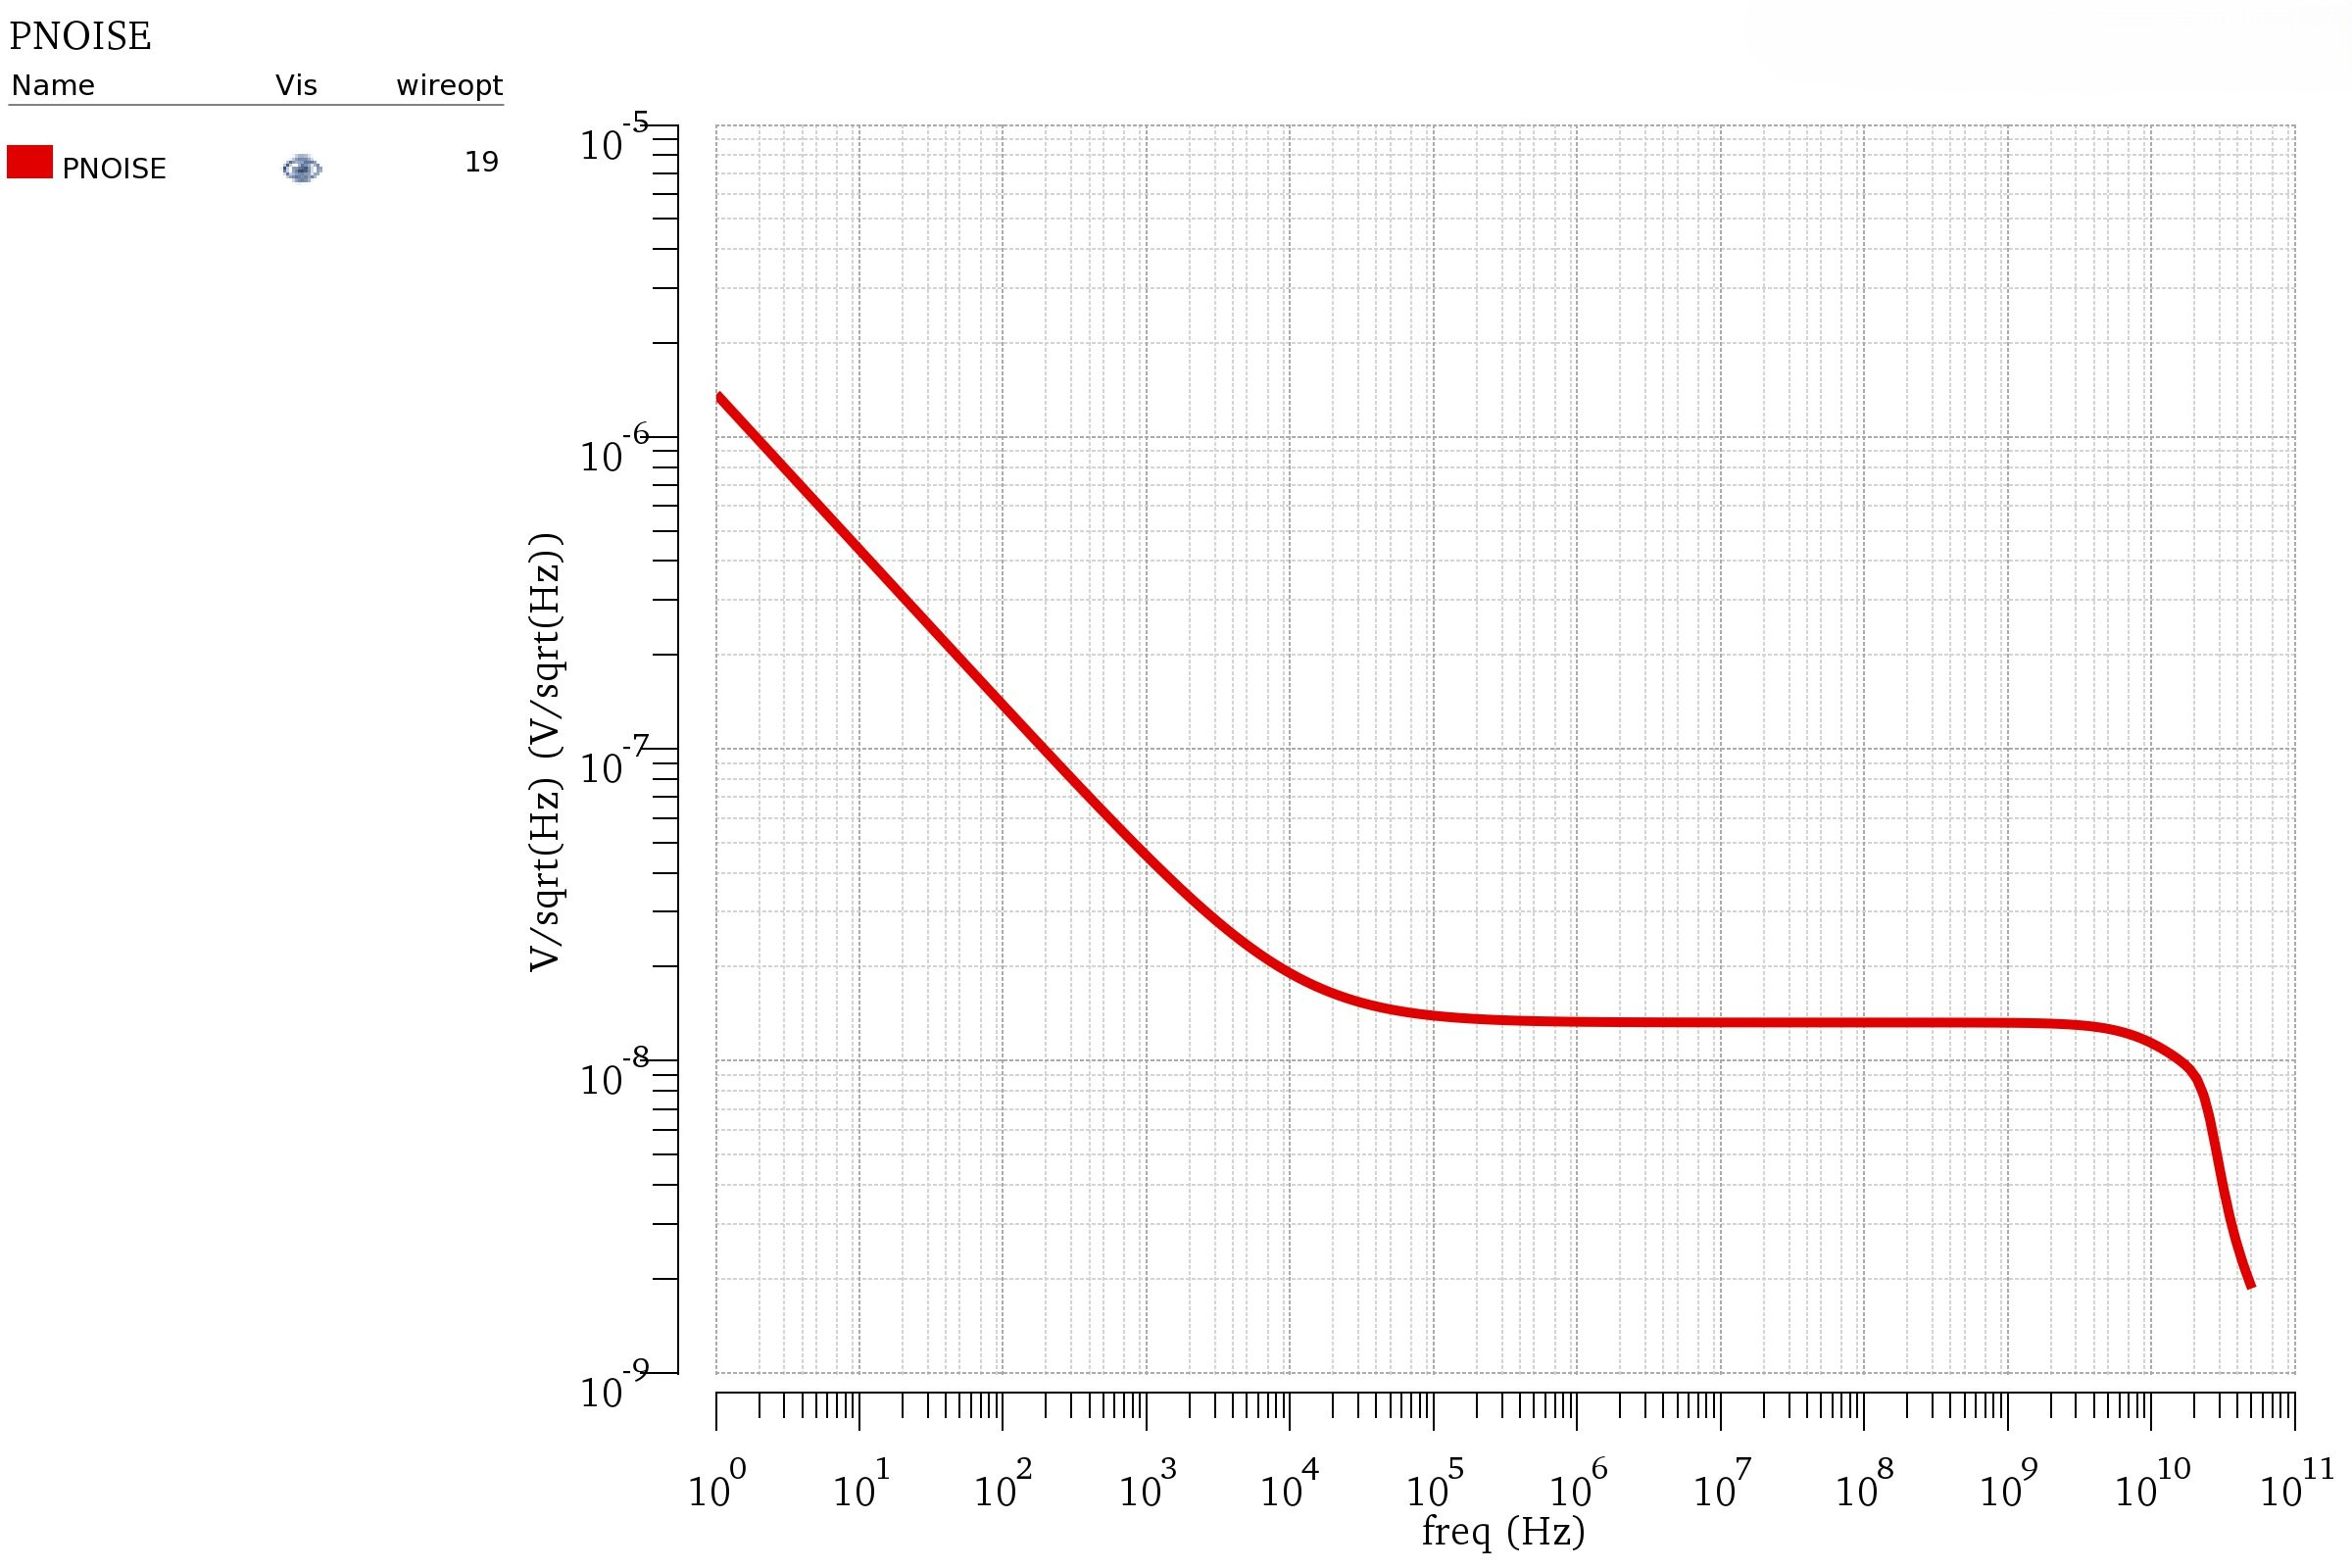
\includegraphics[width=0.9\textwidth]{img/Termination_VGA_img/chain_noise.JPG}} % Replace with Chain Noise Plot
    \caption{Noise spectral density of the entire front-end chain at maximum configurations.}
    \label{fig:chain_noise}
\end{figure}

\begin{table}[H]
    \centering
    \caption{Total Integrated Noise}
    \label{tab:chain_noise}
    \begin{tabular}{@{}ll@{}}
        \toprule
        \textbf{Parameter} & \textbf{Value} \\ 
        \midrule
        Integration Bandwidth & 1 Hz to 16.0 GHz \\ 
        Total Integrated Noise (RMS) & 1.514 mVrms \\ 
        Total Integrated VGA Noise (RMS) & 0.542 mVrms \\
        \bottomrule
    \end{tabular}
\end{table}

\subsubsection*{Chain Linearity}
The end-to-end chain linearity was also verified. Figure \ref{fig:chain_linearity} visualizes the cascaded THD and P1dB limits, proving that the cumulative non-linearities of the input matching network and the VGA do not compress the PAM4 eye structure at nominal input amplitudes.

\begin{figure}[H]
    \centering
    \begin{subfigure}[b]{0.48\textwidth}
        \centering
        \framebox{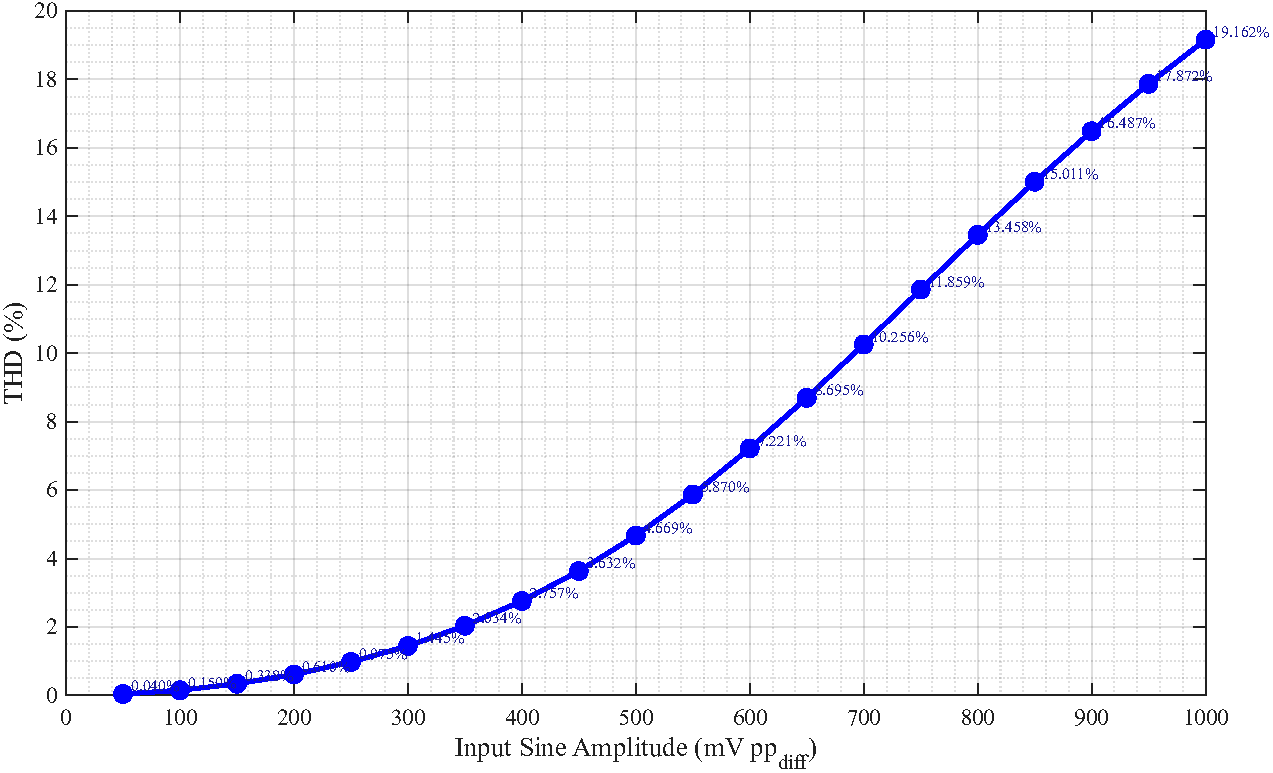
\includegraphics[width=\textwidth]{img/Termination_VGA_img/chain_thd.pdf}} % Replace with Chain THD Plot
        \caption{Total Harmonic Distortion (THD)}
        \label{fig:chain_thd}
    \end{subfigure}
    \hfill
    \begin{subfigure}[b]{0.48\textwidth}
        \centering
        \framebox{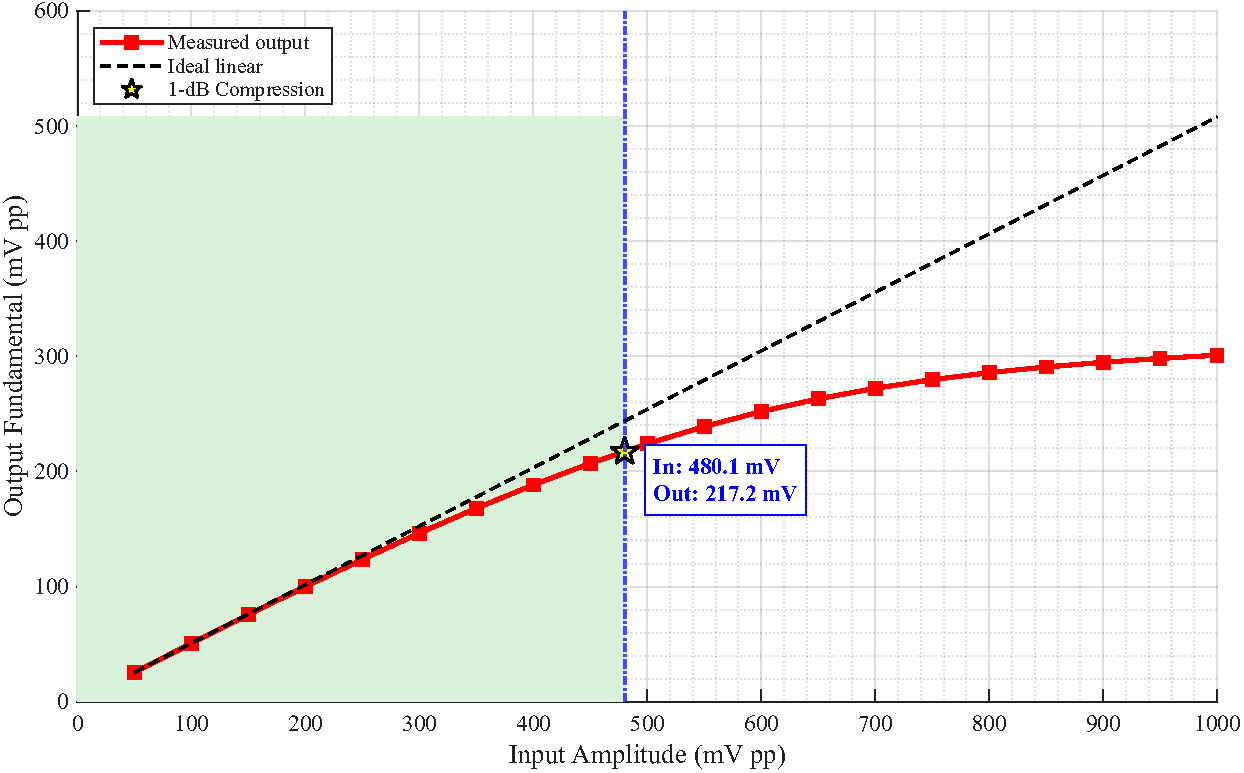
\includegraphics[width=\textwidth]{img/Termination_VGA_img/chain_p1db.pdf}} % Replace with Chain P1dB Plot
        \caption{1-dB Compression Point (P1dB)}
        \label{fig:chain_p1db}
    \end{subfigure}
    \caption{End-to-end chain linearity profiles.}
    \label{fig:chain_linearity}
\end{figure}
